\section{Qualification evidence}\label{app:res-evidence}
\subsection{Measurement records}\label{app:res-provenance}
\begin{table}[H]\centering\small
\begin{tabular}{p{.34\linewidth}p{.58\linewidth}}
\toprule Record & Identity or scope\\\midrule
Physical classifier evidence & 184 paired lines, 14 pages, 5471 reference characters\\
Evaluated reader & joint\_best, SHA-256 prefix \texttt{336802d535992323}\\
Evaluated writer & 11\_pw170, \texttt{1884fb86467538eb}\\
Numerical comparison reader & scratch\_best, \texttt{2add315ded078de5}\\
Numerical comparison writer & 11w\_pw170\_scratch, \texttt{b23a709a30144f67}\\
Checkpoint training provenance & The evaluated joint/pw170 weights use the recorded library training route. Numerical comparison models are listed separately.\\
Execution records & Physical motion and request timings are ODROID records. Saved-image scoring and geometric analyses are offline verification on the development host.\\
\bottomrule\end{tabular}
\caption{Identities and scope of the retained measurements.}\label{tab:app-checkpoints}\end{table}
\subsection{Original-handwriting classifier evidence}\label{app:res-validation}
\begin{table}[H]\centering\small
\begin{tabular}{lrrrr}\toprule
\textbf{Evaluation set} & \textbf{Lines} & \textbf{Characters} & \textbf{Joint / \%} & \textbf{NumPy / \%}\\\midrule
Public IAM validation & 976 & 42072 & 94.12 & 94.39\\
Photographed A & 31 & 934 & 94.00 & 94.65\\
Photographed B & 19 & 739 & 95.81 & 97.70\\
Photographed O & 22 & 1017 & 94.40 & 94.79\\
Photographed T & 11 & 345 & 85.51 & 89.28\\
Photographed Y & 17 & 640 & 92.03 & 92.50\\
All & 1076 & 45747 & 94.06 & 94.39\\
\bottomrule\end{tabular}
\caption{Reader character accuracy by validation population.}\label{tab:app-reader-breakdown}
\end{table}
The complete author confusion matrix is shown in QTP2.
\subsection{Reproduced-page classifier evidence}\label{app:res-page-records}
The text and author classifier results are in QTP1. The following breakdown retains the three tested text blocks.
\begin{table}[!htbp]\centering\small
\begin{tabular}{lrrrr}\toprule
\textbf{Text block} & \textbf{Lines} & \textbf{Characters} & \textbf{Character / \%} & \textbf{Writer / \%}\\\midrule
Paragraph & 119 & 4041 & 84.88 & 91.60\\
Pangram & 21 & 463 & 78.40 & 76.19\\
Source text & 44 & 967 & 85.32 & 77.27\\
All & 184 & 5471 & 84.41 & 86.41\\
\bottomrule\end{tabular}
\caption{Physical reproduction scores by text block.}\label{tab:res-r1-blocks}
\end{table}

\subsection{Geometric comparison evidence}\label{app:res-geometric}
The following values support QTP1's natural-variation comparison. They use the same original reference banks for genuine and robot probes.
\begin{table}[H]\centering\small
\begin{tabular}{lrrrrr}
\toprule Writer & Words & Genuine F / \% & Robot F / \% & Relative / \% & Nearest / \%\\\midrule
150 & 8 & 90.01 & 87.73 & 97.47 & 97.26\\
152 & 8 & 91.61 & 74.99 & 81.86 & 83.63\\
153 & 6 & 89.24 & 74.12 & 83.05 & 82.90\\
384 & 6 & 80.14 & 72.34 & 90.27 & 88.99\\
552 & 8 & 79.92 & 61.95 & 77.51 & 83.54\\
588 & 5 & 75.66 & 64.16 & 84.80 & 91.36\\
A & 12 & 72.98 & 60.40 & 82.76 & 82.40\\
B & 10 & 74.11 & 69.70 & 94.05 & 93.83\\
O & 5 & 76.03 & 70.22 & 92.36 & 97.50\\
T & 4 & 66.24 & 49.19 & 74.26 & 70.34\\
Y & 11 & 77.99 & 74.16 & 95.10 & 95.09\\
\bottomrule\end{tabular}
\caption{All writers in the repeated-word comparison.}\label{tab:app-geometric-writers}\end{table}
Figures~\ref{fig:app-geometry-dylan} to~\ref{fig:app-geometry-153} show further retained comparisons. Each left column compares two genuine samples. Each right column compares a robot word with its selected genuine reference. The printed F-scores are individual nearest-reference examples, rather than the ordinary-reference writer averages.
\begin{figure}[!htbp]\centering
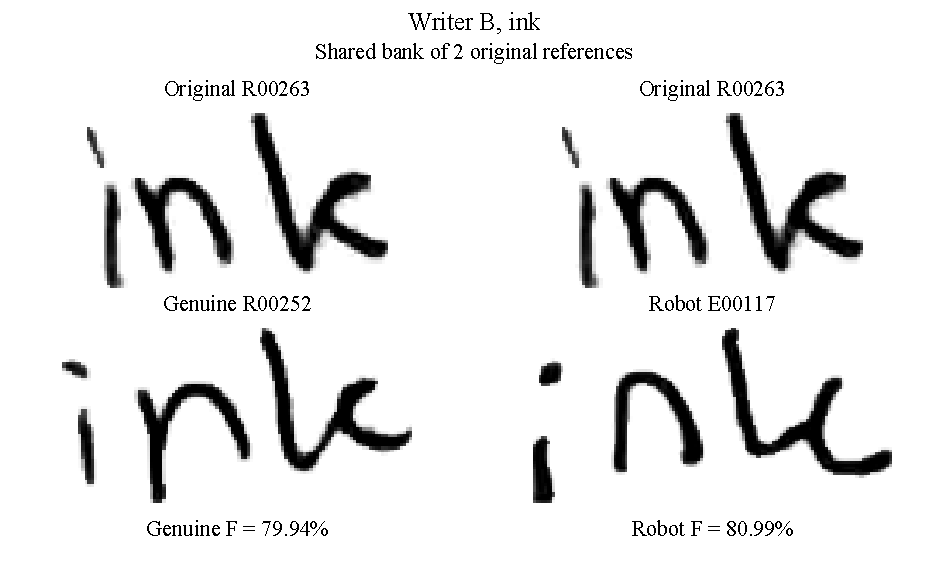
\includegraphics[width=\linewidth]{Figures/GeometricEvidence/comparison_dylan_crops.pdf}
\caption{Genuine and robot word comparisons for writer B.}\label{fig:app-geometry-dylan}\end{figure}
\begin{figure}[!htbp]\centering
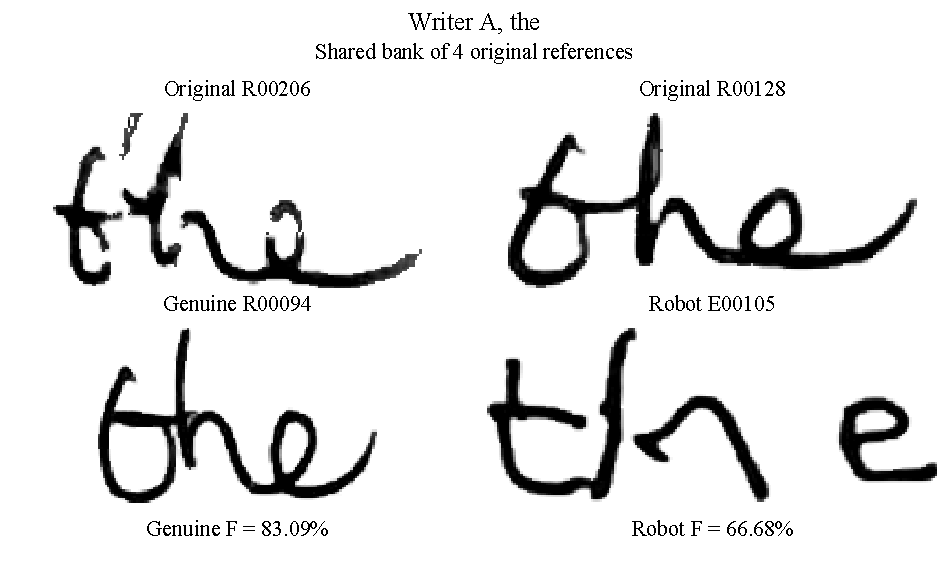
\includegraphics[width=\linewidth]{Figures/GeometricEvidence/comparison_abhinav_crops.pdf}
\caption{Genuine and robot word comparisons for writer A.}\label{fig:app-geometry-abhinav}\end{figure}
\begin{figure}[!htbp]\centering
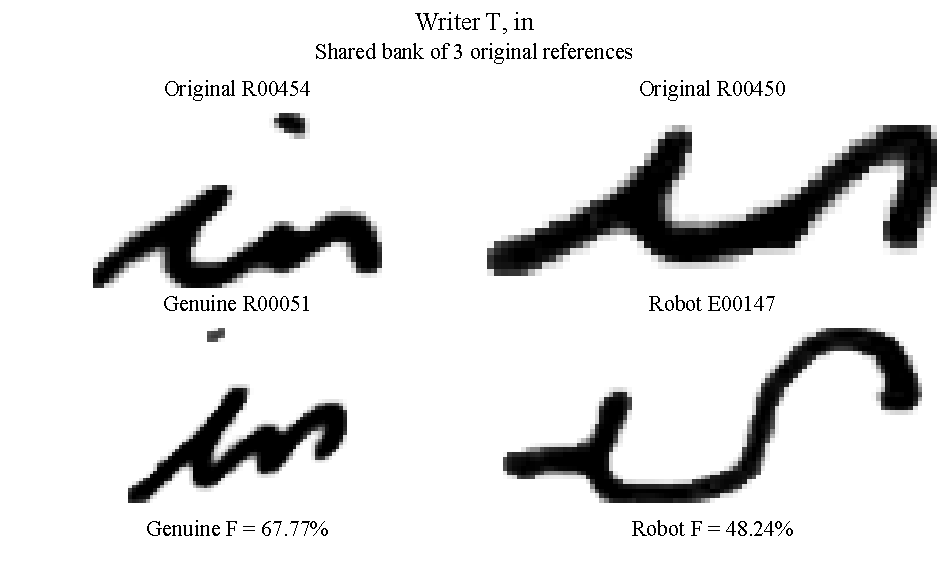
\includegraphics[width=\linewidth]{Figures/GeometricEvidence/comparison_thiya_crops.pdf}
\caption{Genuine and robot word comparisons for writer T.}\label{fig:app-geometry-thiya}\end{figure}
\begin{figure}[!htbp]\centering
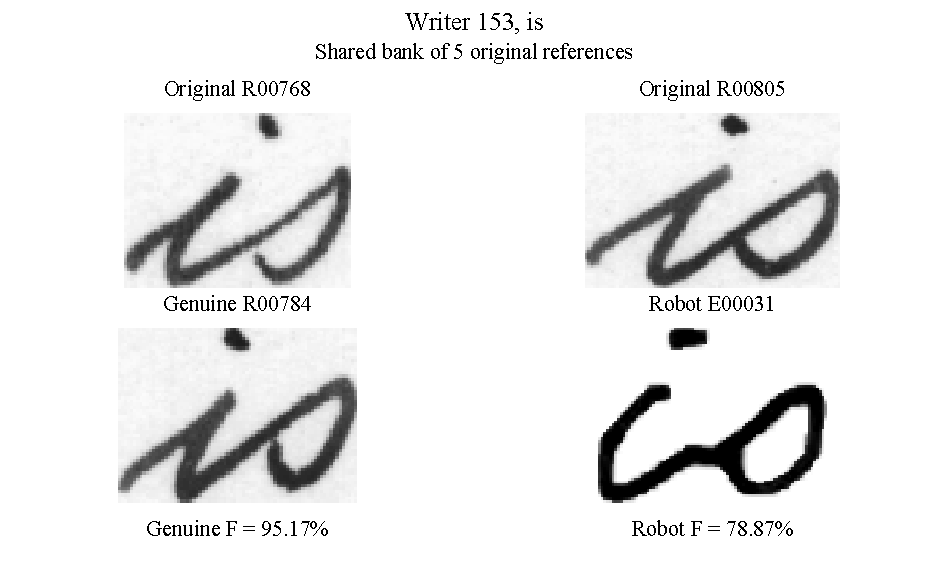
\includegraphics[width=\linewidth]{Figures/GeometricEvidence/comparison_153_crops.pdf}
\caption{Genuine and robot word comparisons for writer 153.}\label{fig:app-geometry-153}\end{figure}
\FloatBarrier
\subsection{Completed reproduction timing records}\label{app:res-speed}
\begin{longtable}{rrrrrr}
\caption{All confirmed ODROID reproduction timings.}\label{tab:app-complete-timings}\\
\toprule Log line & Characters & Synthesis / s & Drawing / s & Total / s & s per character\\\midrule\endfirsthead
\toprule Log line & Characters & Synthesis / s & Drawing / s & Total / s & s per character\\\midrule\endhead
32 & 378 & 8.23 & 497.55 & 507.57 & 1.343\\
185 & 378 & 17.98 & 637.31 & 657.72 & 1.740\\
203 & 43 & 17.66 & 92.59 & 110.59 & 2.572\\
595 & 91 & 16.44 & 175.50 & 192.47 & 2.115\\
631 & 378 & 12.36 & 651.18 & 665.14 & 1.760\\
682 & 43 & 14.80 & 91.30 & 106.44 & 2.475\\
718 & 82 & 17.06 & 165.46 & 183.04 & 2.232\\
816 & 378 & 39.27 & 899.55 & 941.48 & 2.491\\
864 & 43 & 20.34 & 113.94 & 134.65 & 3.131\\
887 & 82 & 27.53 & 204.05 & 232.16 & 2.831\\
1004 & 378 & 58.78 & 1022.83 & 1085.01 & 2.870\\
1027 & 43 & 26.52 & 139.66 & 166.61 & 3.875\\
1050 & 82 & 33.67 & 225.88 & 260.33 & 3.175\\
1099 & 378 & 16.63 & 839.33 & 859.00 & 2.272\\
1122 & 43 & 18.81 & 106.99 & 126.19 & 2.935\\
1145 & 75 & 25.39 & 162.76 & 188.60 & 2.515\\
1189 & 378 & 12.11 & 663.01 & 676.64 & 1.790\\
1225 & 43 & 15.10 & 96.53 & 112.00 & 2.605\\
1260 & 43 & 15.22 & 96.44 & 112.03 & 2.605\\
1348 & 378 & 104.08 & 656.92 & 762.84 & 2.018\\
1384 & 43 & 15.65 & 81.40 & 97.28 & 2.262\\
1407 & 91 & 23.34 & 198.59 & 222.63 & 2.446\\
1495 & 378 & 14.17 & 726.40 & 742.72 & 1.965\\
1518 & 43 & 15.19 & 95.64 & 111.18 & 2.586\\
1541 & 132 & 22.88 & 254.16 & 277.90 & 2.105\\
\bottomrule\end{longtable}
\subsection{Recorded classification stages}\label{app:res-classification-time}
\begin{table}[!htbp]\centering\small
\begin{tabular}{lrr}\toprule
\textbf{Recorded quantity} & \textbf{500 characters} & \textbf{982 characters}\\\midrule
Loading / s & 0.63 & 0.53\\
Conditioning / s & 6.61 & 6.04\\
Segmentation / s & 4.29 & 5.59\\
Cropping / s & 4.61 & 4.65\\
Image stages / s & 16.14 & 16.81\\
Reading / s & 19.02 & 24.66\\
Writer classification / s & 11.09 & 14.01\\
Network stages / s & 30.12 & 38.67\\
Total / s & 46.26 & 55.49\\
R4 allowance / s & 14.50 & 26.55\\
Overrun / s & 31.76 & 28.94\\
\bottomrule\end{tabular}
\caption{Recorded ODROID classification-stage timings.}\label{tab:res-r4-times}
\end{table}

\subsection{Dimensional measurement evidence}\label{app:res-geometry-calculation}
QTP5 shows all 70 signed errors. These statistics retain the ten readings per feature. The supplied readings are retained in the measurement archive.
\begin{table}[H]\centering\small
\begin{tabular}{lrrrr}
\toprule Feature & Mean / mm & Sample SD / mm & Min / mm & Max / mm\\\midrule
Square bottom X & +0.150 & 0.315 & -0.40 & +0.48\\
Square top X & +0.112 & 0.277 & -0.34 & +0.42\\
Square left Y & -0.018 & 0.342 & -0.46 & +0.44\\
Square right Y & -0.006 & 0.304 & -0.42 & +0.40\\
Triangle base & +0.130 & 0.315 & -0.42 & +0.46\\
Triangle left slope & -0.182 & 0.327 & -0.49 & +0.43\\
Triangle right slope & +0.182 & 0.327 & -0.43 & +0.49\\
\bottomrule\end{tabular}
\caption{Repeated feature-length error statistics, ten readings per feature.}\label{tab:app-gantry-features}\end{table}
\subsection{Stored profile evidence}\label{app:res-inventory}
\begin{table}[H]\centering\small
\begin{tabular}{lrr}
\toprule Writer & Character mappings & Physical pages\\\midrule
150 & 42 & 1\\
152 & 38 & 1\\
153 & 37 & 2\\
384 & 36 & 2\\
552 & 40 & 1\\
588 & 41 & 1\\
A & 56 & 2\\
B & 42 & 1\\
O & 43 & 1\\
T & 42 & 1\\
Y & 58 & 1\\
\bottomrule\end{tabular}
\caption{Stored profiles and physical-page coverage.}\label{tab:app-style-inventory}\end{table}
\subsection{Training log extracts}\label{app:training-records}
Selected rows from the supplied first-principles logs are retained below. Full transcribed training records remain in the accompanying evidence archive.
\begin{longtable}{rrrr}
\caption{Selected writer training log records.}\label{tab:app-author-log}\\
\toprule Epoch & Loss & Validation / \% & Time / min\\\midrule\endfirsthead
\toprule Epoch & Loss & Validation / \% & Time / min\\\midrule\endhead
1 & 1.979 & 47.7 & 20.1\\
10 & 0.531 & 87.7 & 20.1\\
18 & 0.378 & 94.2 & 20.6\\
31 & 0.154 & 95.5 & 19.6\\
41 & 0.068 & 96.8 & 19.5\\
47 & 0.082 & 96.8 & 20.9\\
\bottomrule\end{longtable}
\begin{longtable}{rrrrrr}
\caption{Selected reader training log records.}\label{tab:app-reader-log}\\
\toprule Epoch & Train loss & Val loss & Val char / \% & Personal / \% & Time / min\\\midrule\endfirsthead
\toprule Epoch & Train loss & Val loss & Val char / \% & Personal / \% & Time / min\\\midrule\endhead
7 & 45.339 & 44.488 & 70.17 & 66.56 & 122.3\\
8 & 24.865 & 18.597 & 87.62 & 88.54 & 120.1\\
11 & 12.862 & 13.298 & 91.43 & 91.40 & 111.6\\
16 & 7.045 & 11.663 & 92.89 & 93.09 & 112.3\\
\bottomrule\end{longtable}
\subsection{Complete physical-page photographs}\label{app:res-physical-pages}
Figures~\ref{fig:app-physical-pages-1} to~\ref{fig:app-physical-pages-7} retain all fourteen photographed output pages.
\begin{figure}[!htbp]\centering
\begin{minipage}{.48\linewidth}\centering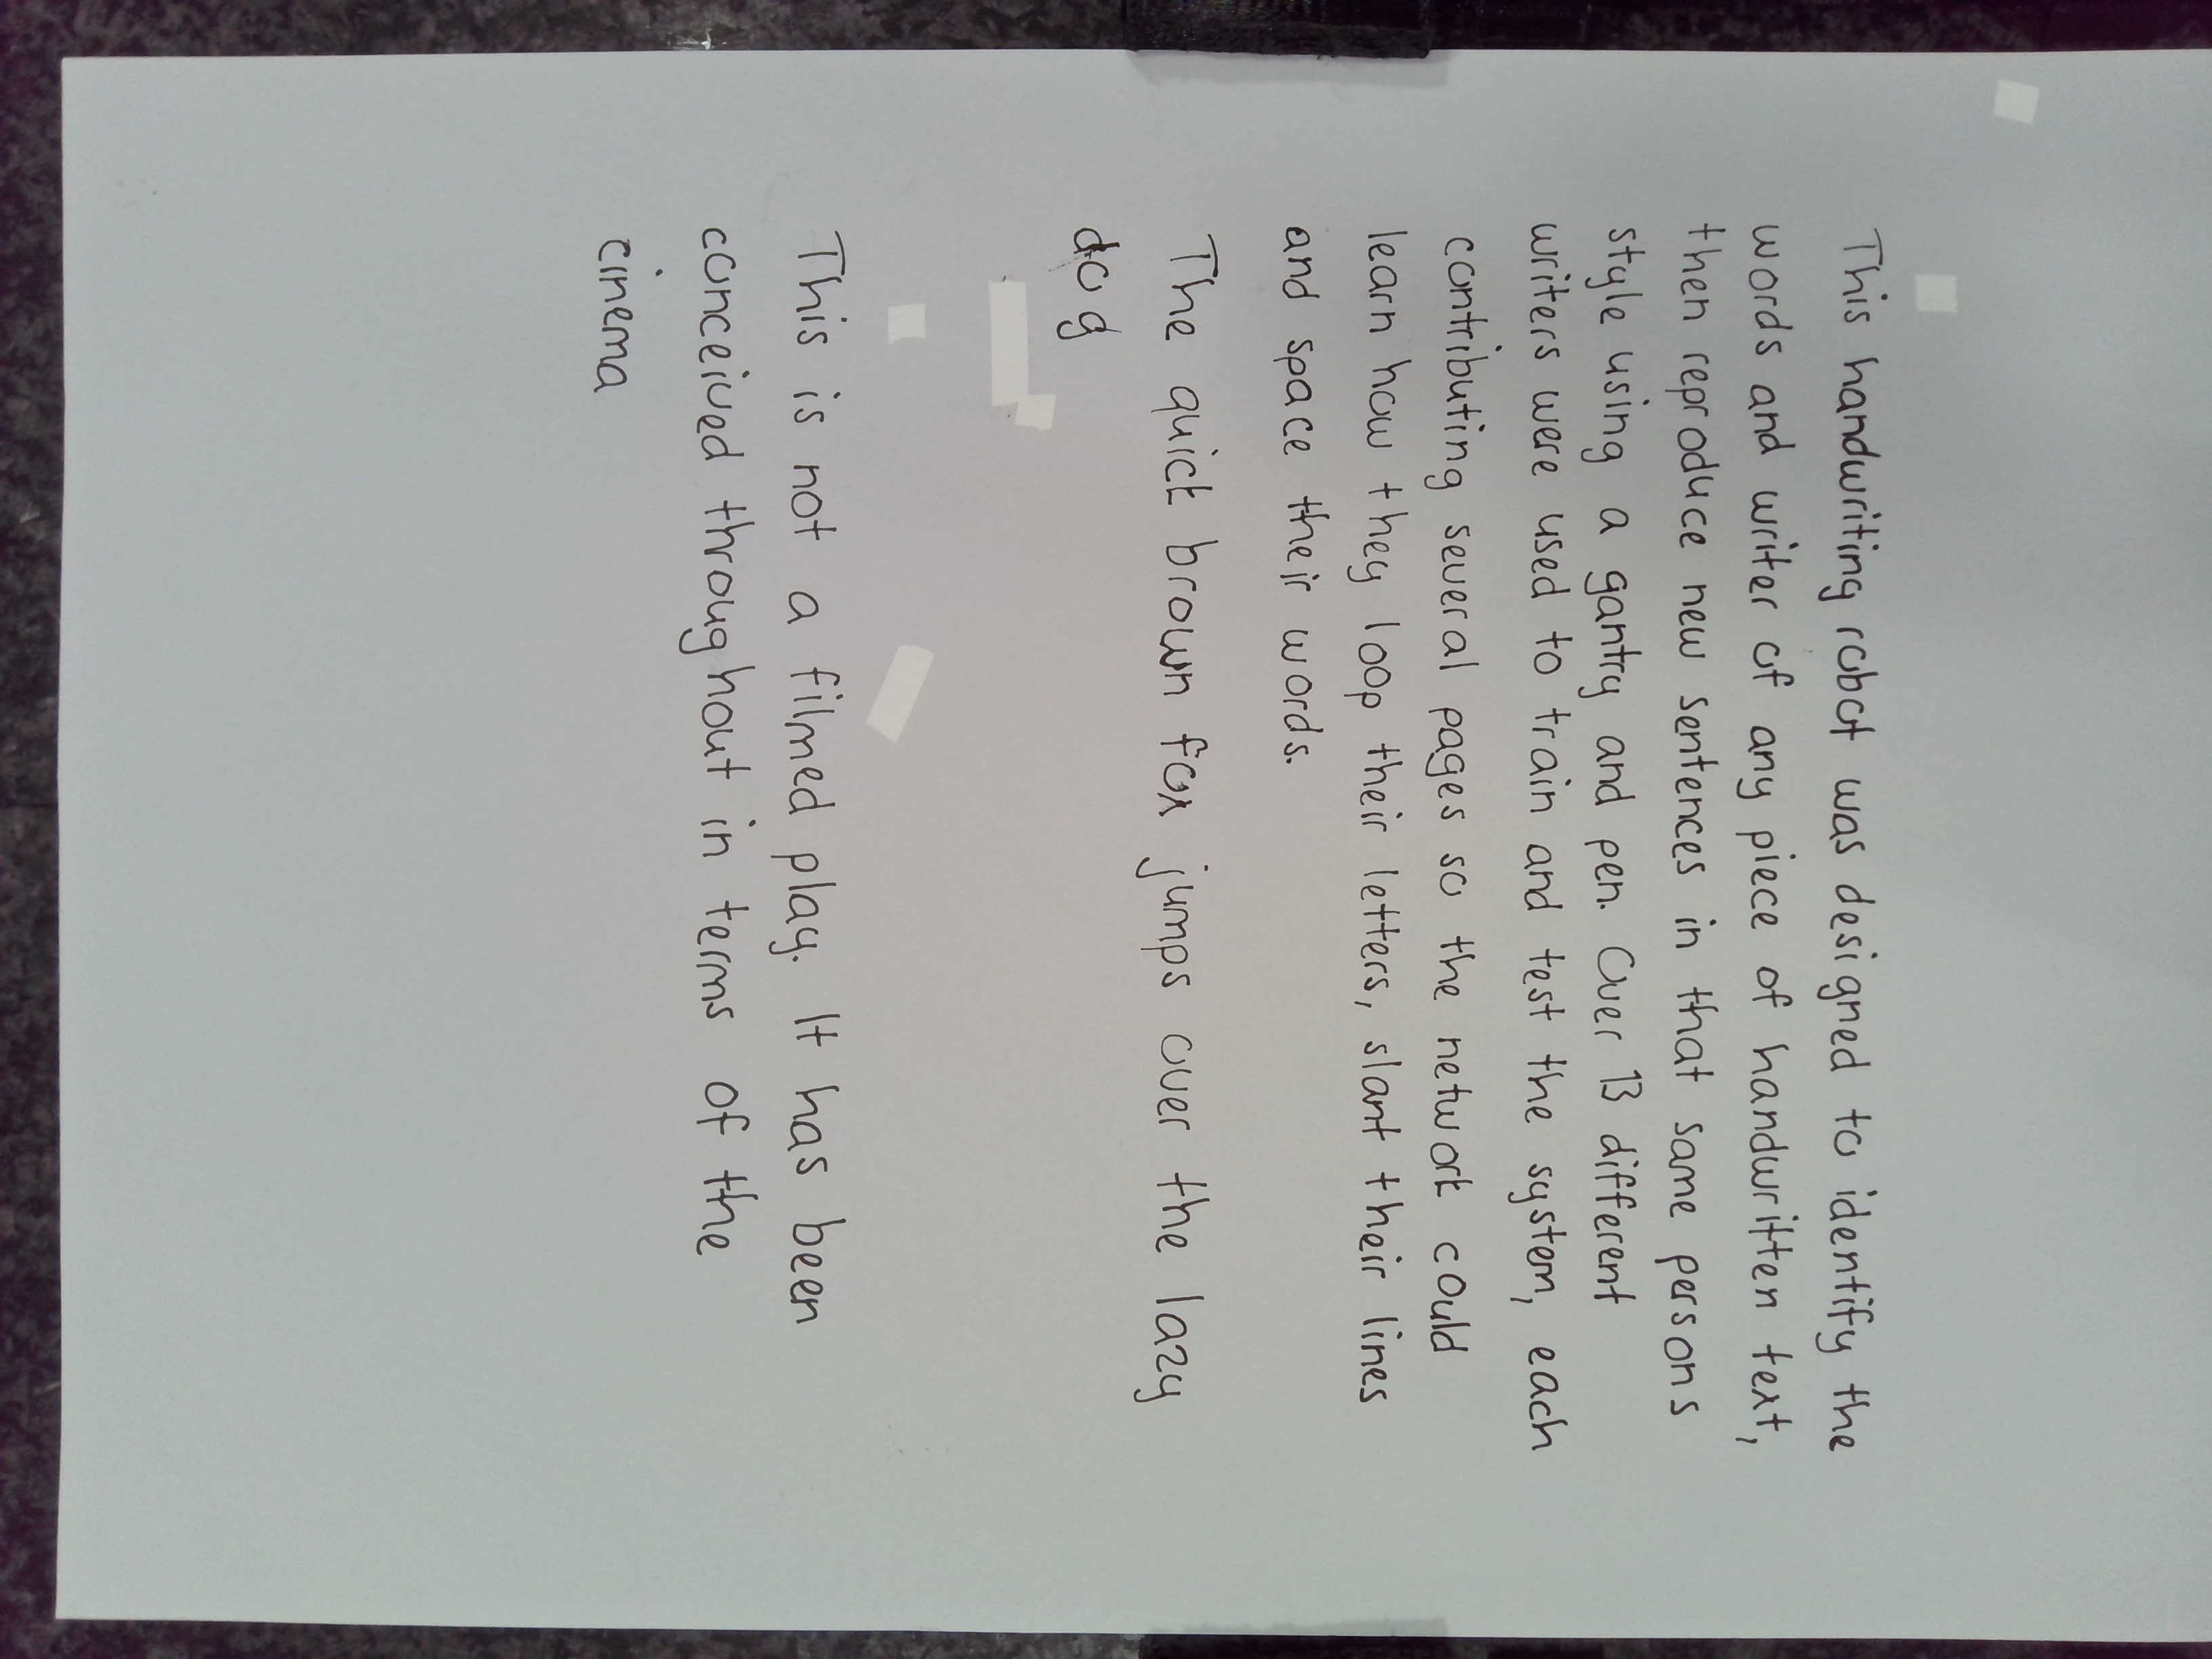
\includegraphics[angle=90,width=\linewidth,height=.55\textheight,keepaspectratio]{Figures/PhysicalPages/Author150.jpg}\par Author150\end{minipage}\hfill
\begin{minipage}{.48\linewidth}\centering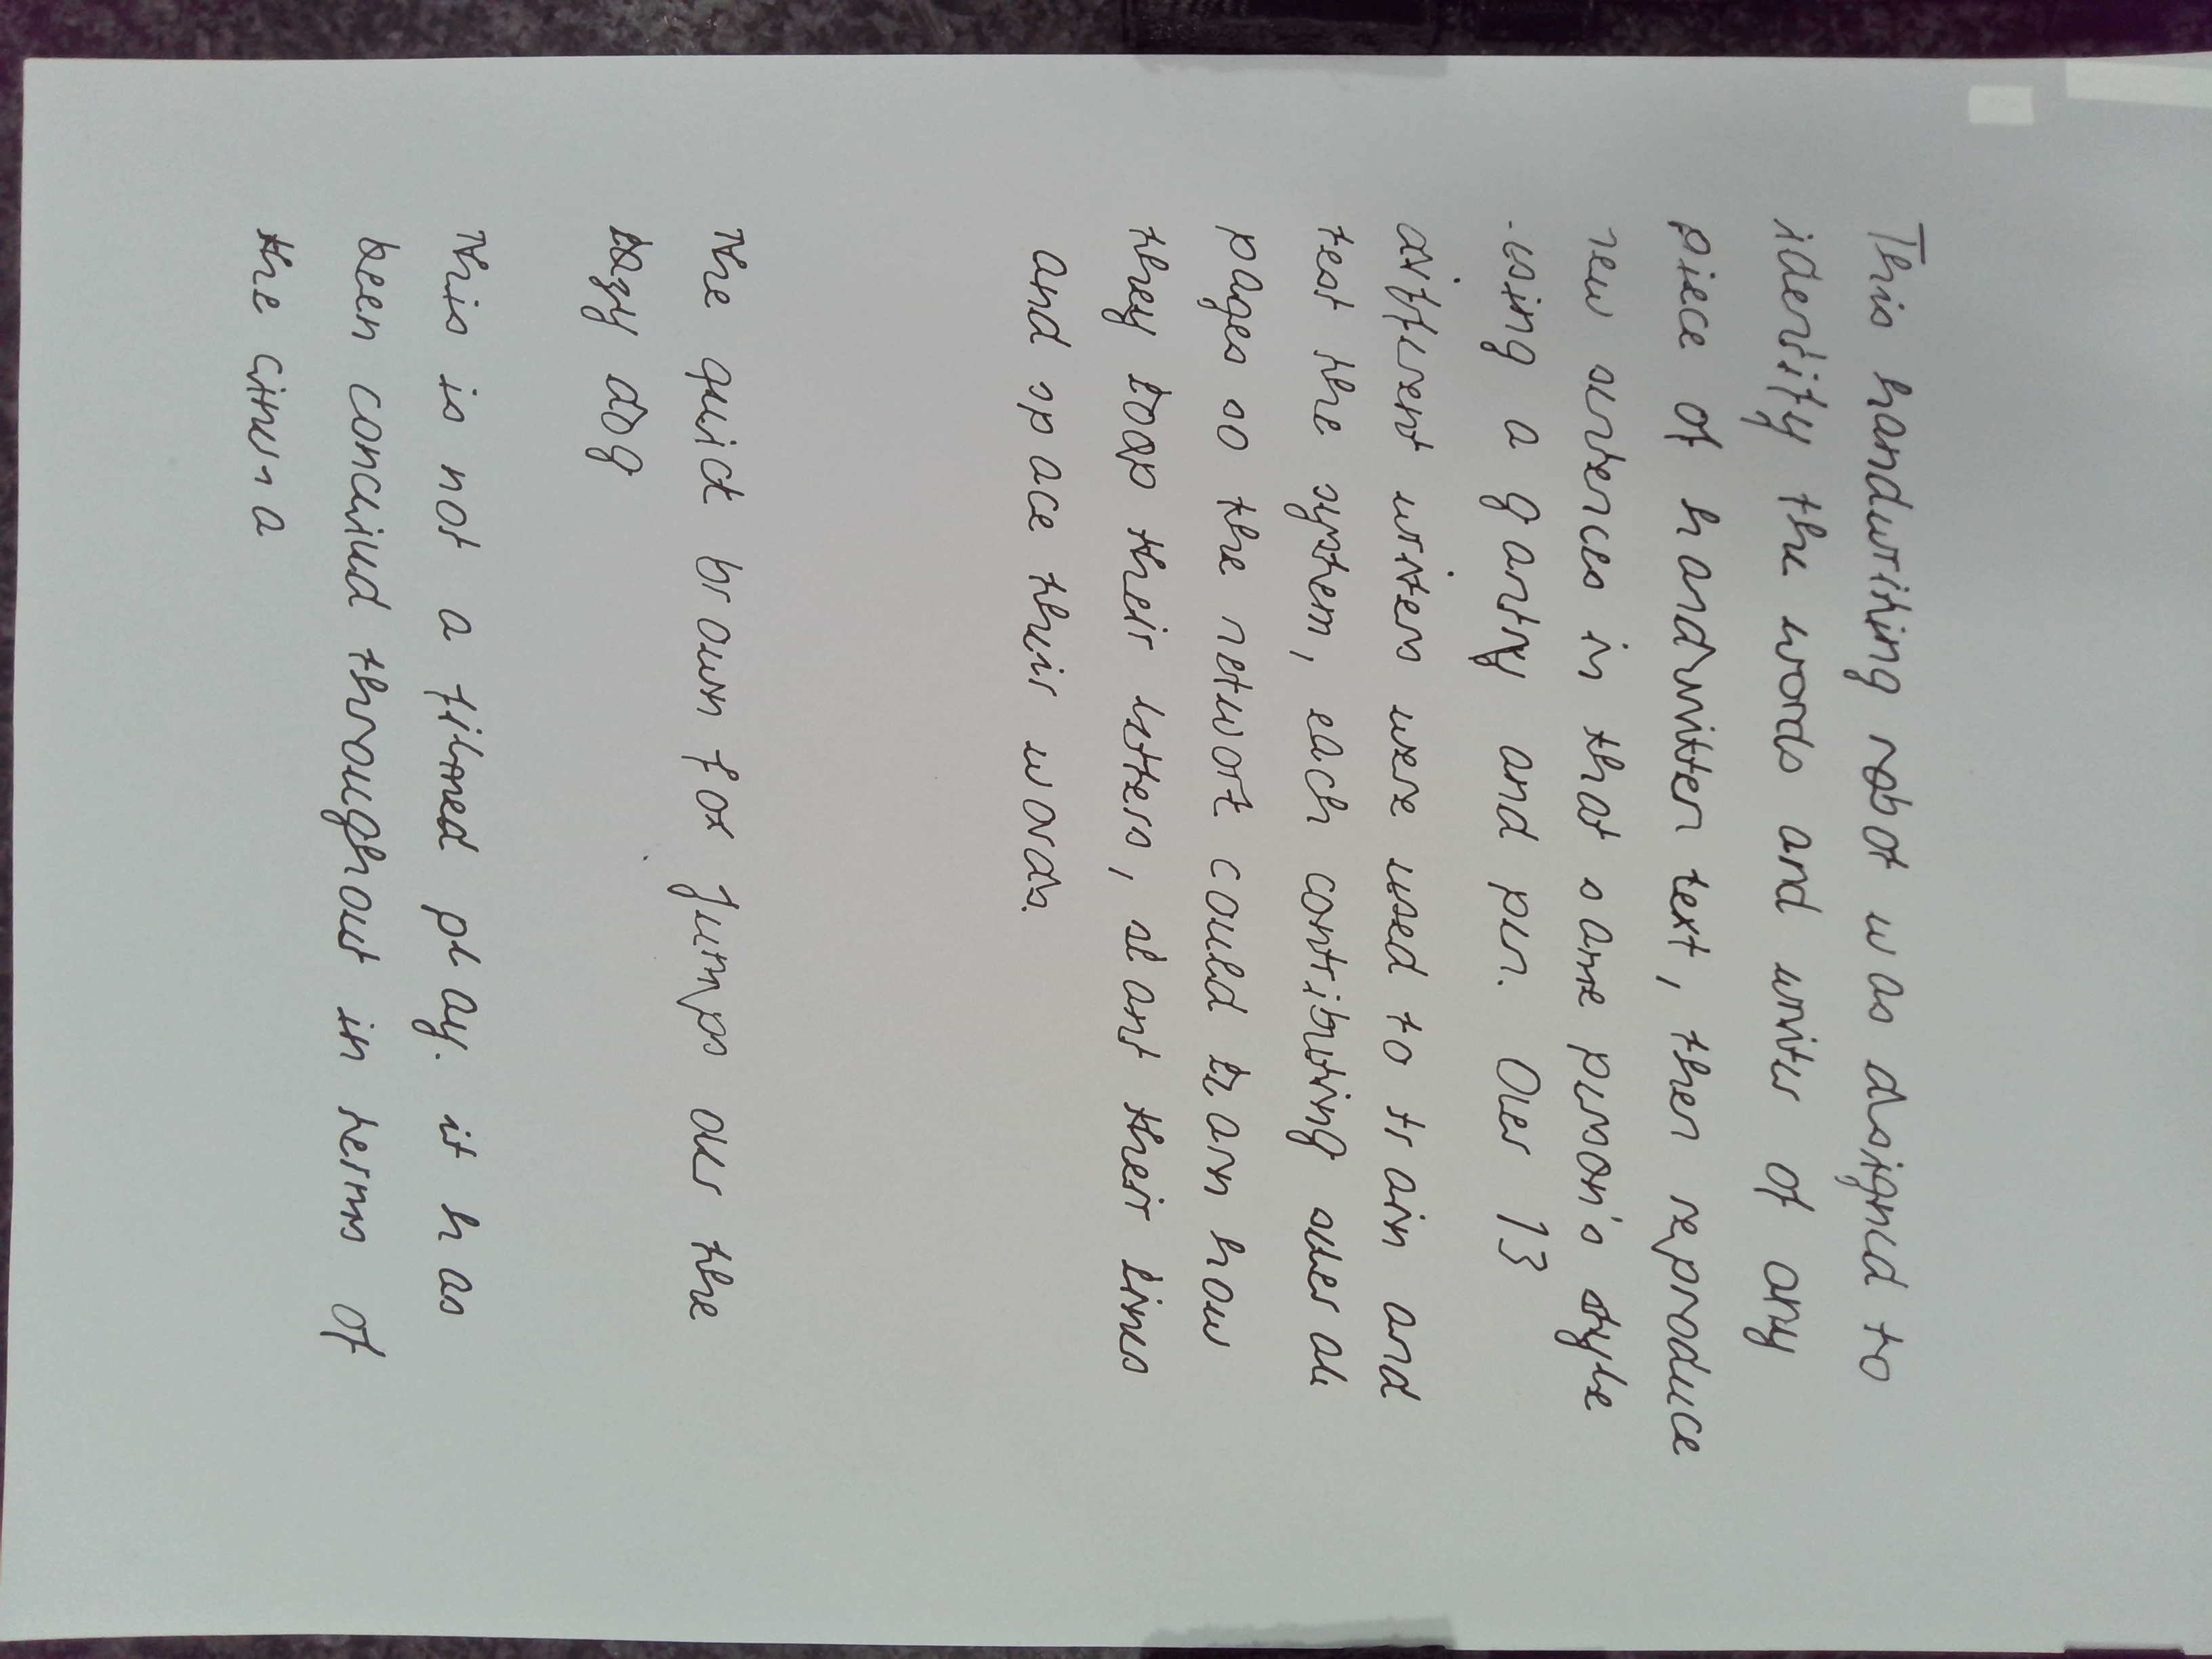
\includegraphics[angle=90,width=\linewidth,height=.55\textheight,keepaspectratio]{Figures/PhysicalPages/Author152.jpg}\par Author152\end{minipage}\hfill
\caption{Physical pages Author150, Author152.}\label{fig:app-physical-pages-1}\end{figure}
\begin{figure}[!htbp]\centering
\begin{minipage}{.48\linewidth}\centering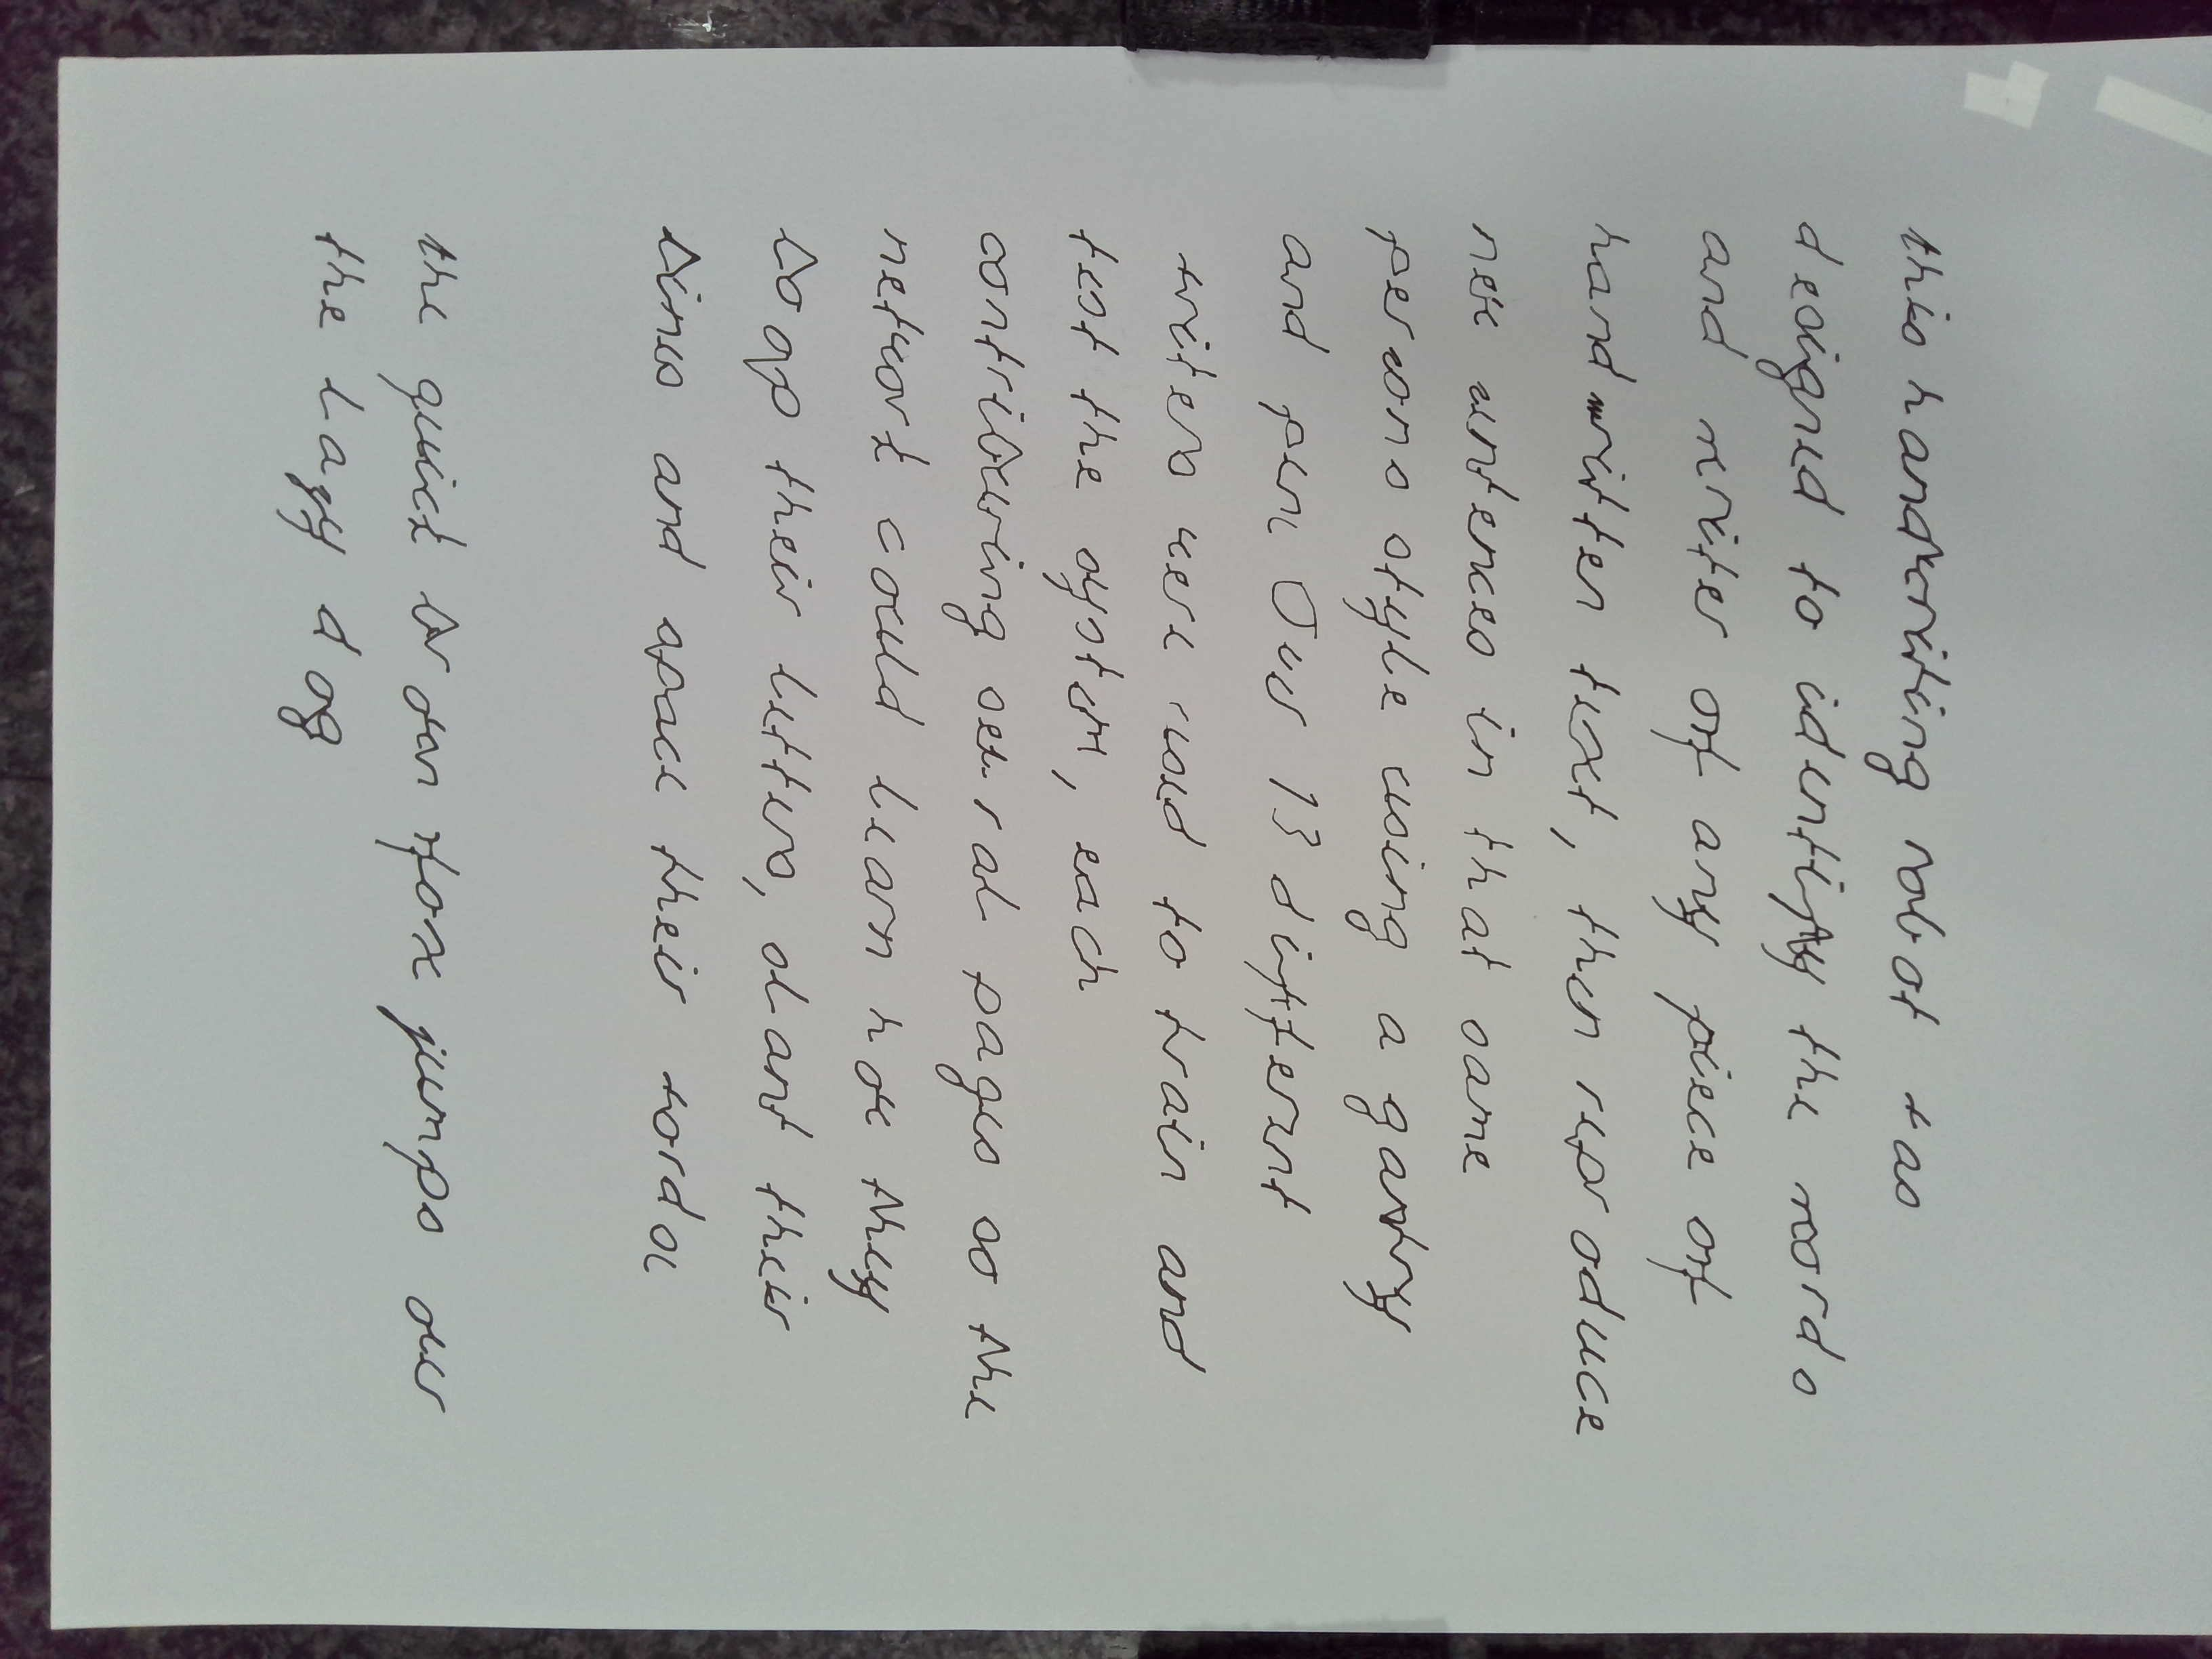
\includegraphics[angle=90,width=\linewidth,height=.55\textheight,keepaspectratio]{Figures/PhysicalPages/Author1531.jpg}\par Author1531\end{minipage}\hfill
\begin{minipage}{.48\linewidth}\centering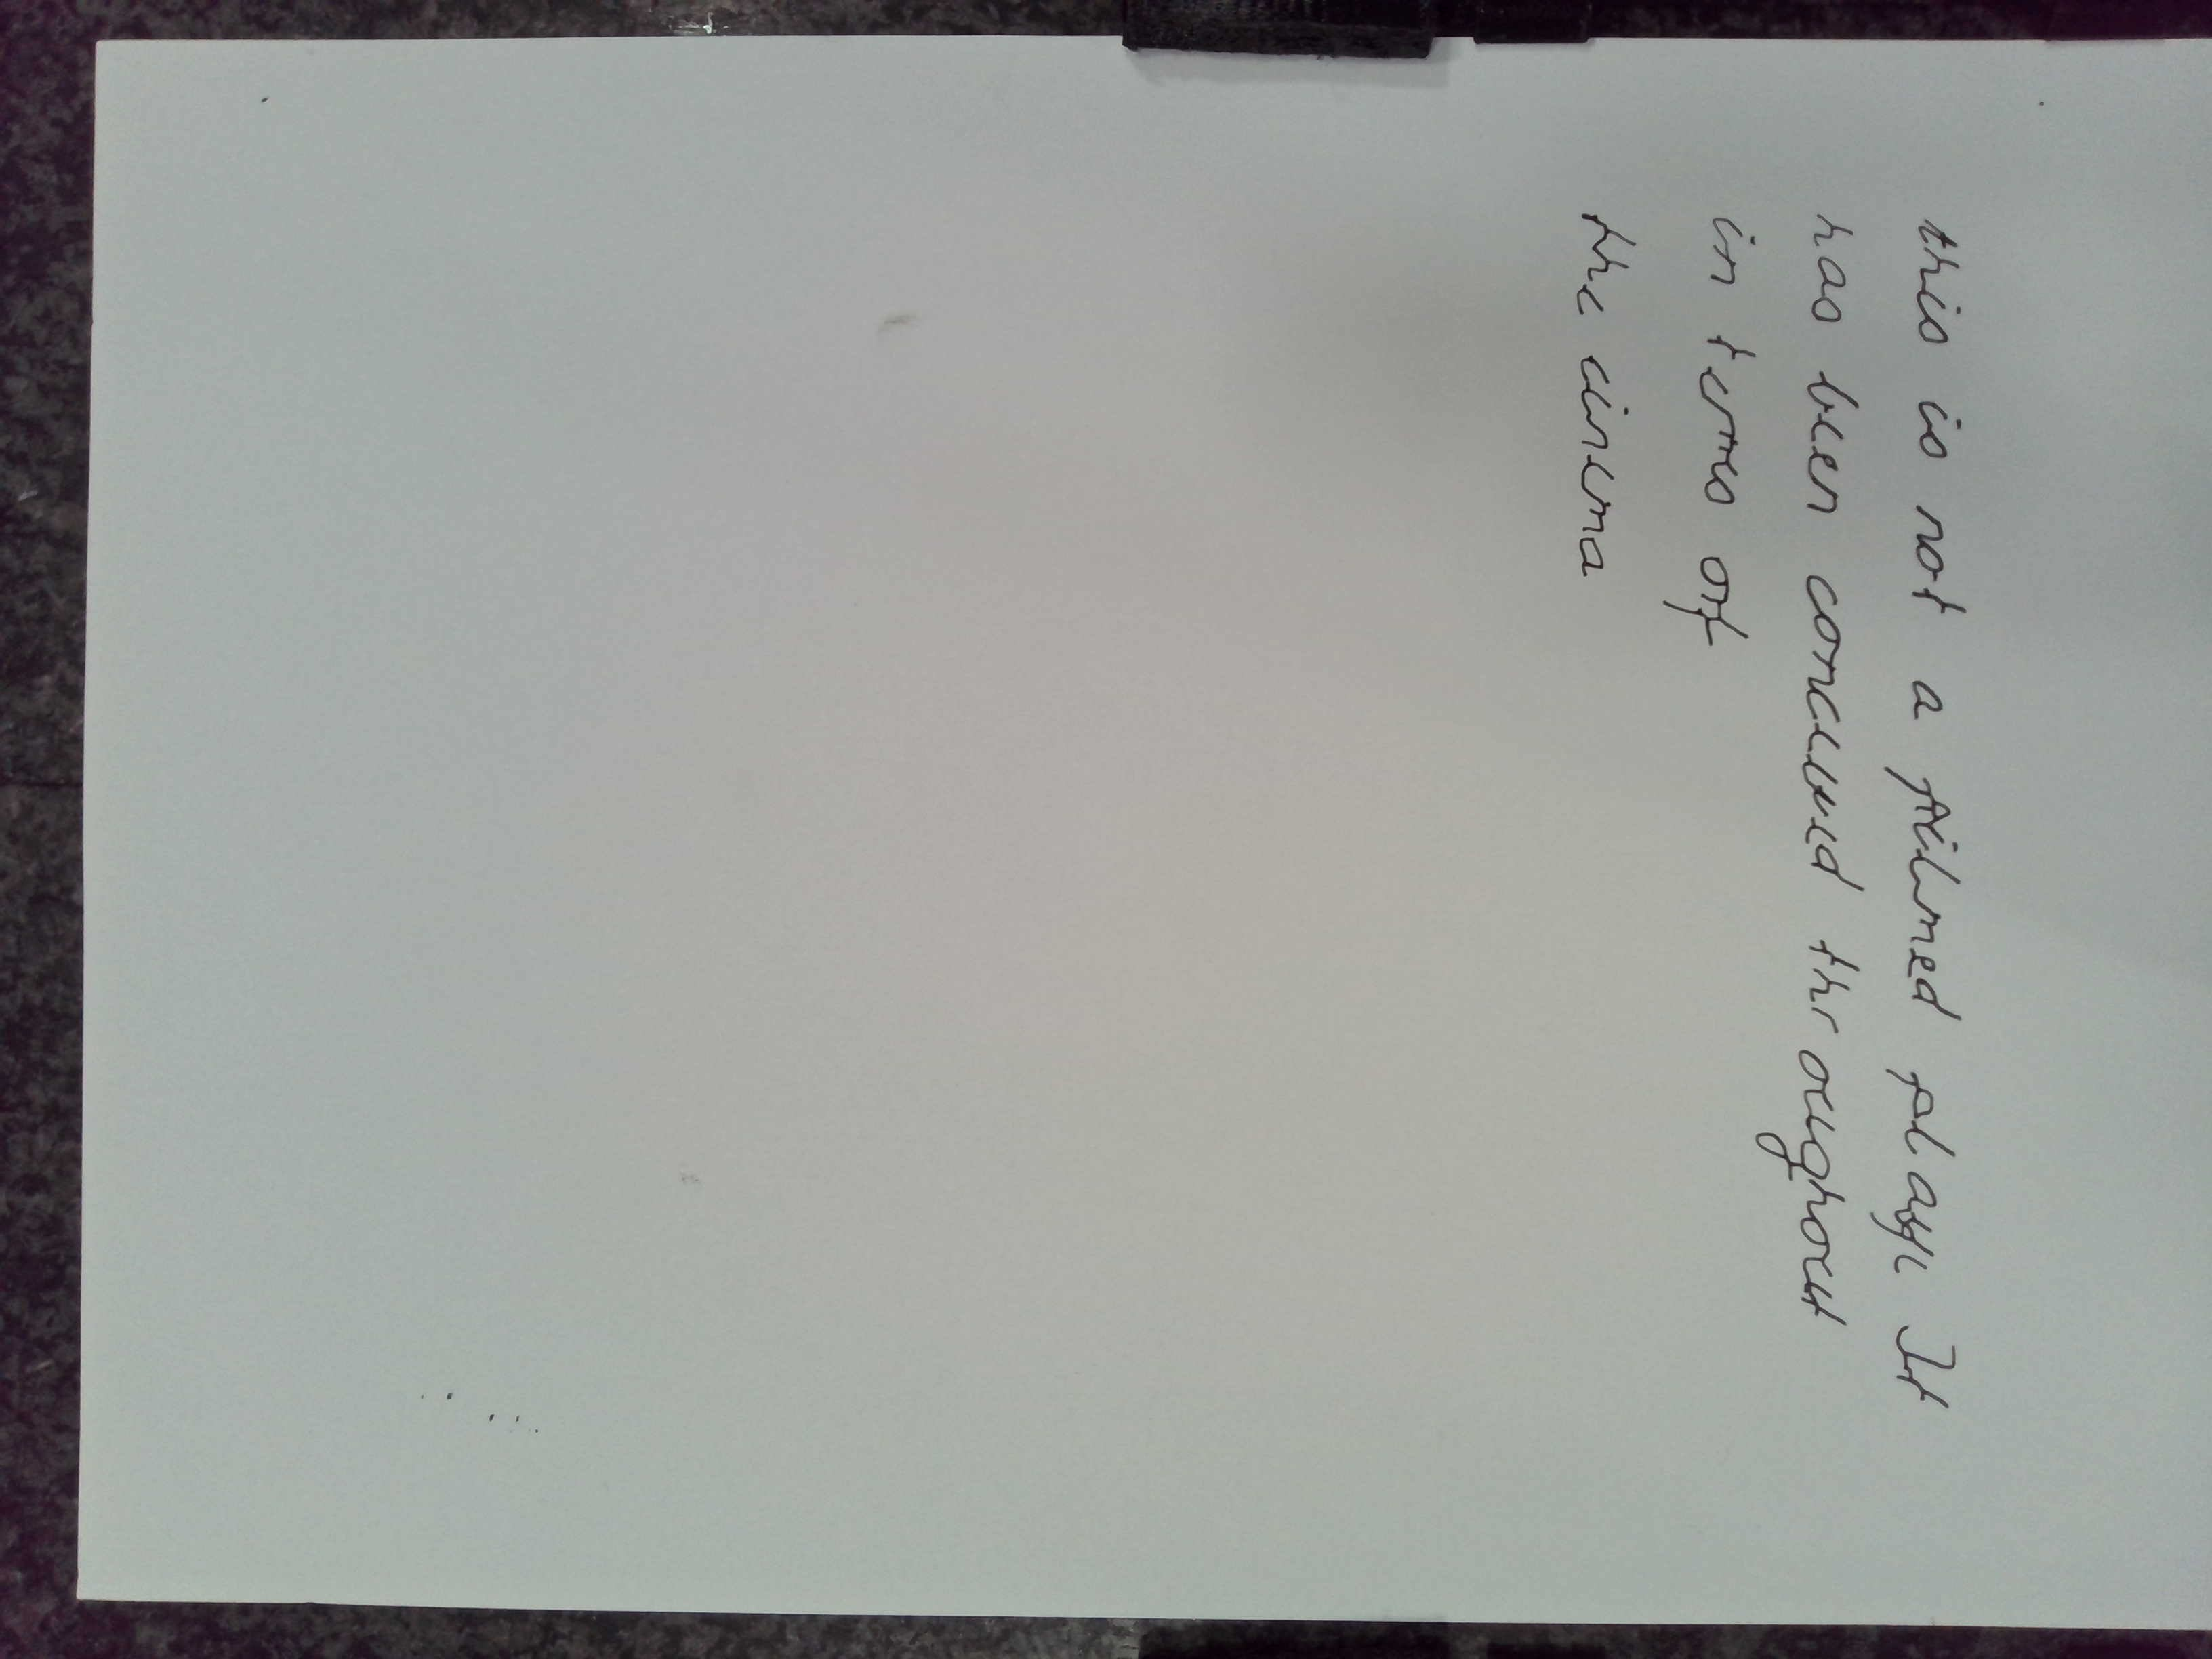
\includegraphics[angle=90,width=\linewidth,height=.55\textheight,keepaspectratio]{Figures/PhysicalPages/Author1532.jpg}\par Author1532\end{minipage}\hfill
\caption{Physical pages Author1531, Author1532.}\label{fig:app-physical-pages-2}\end{figure}
\begin{figure}[!htbp]\centering
\begin{minipage}{.48\linewidth}\centering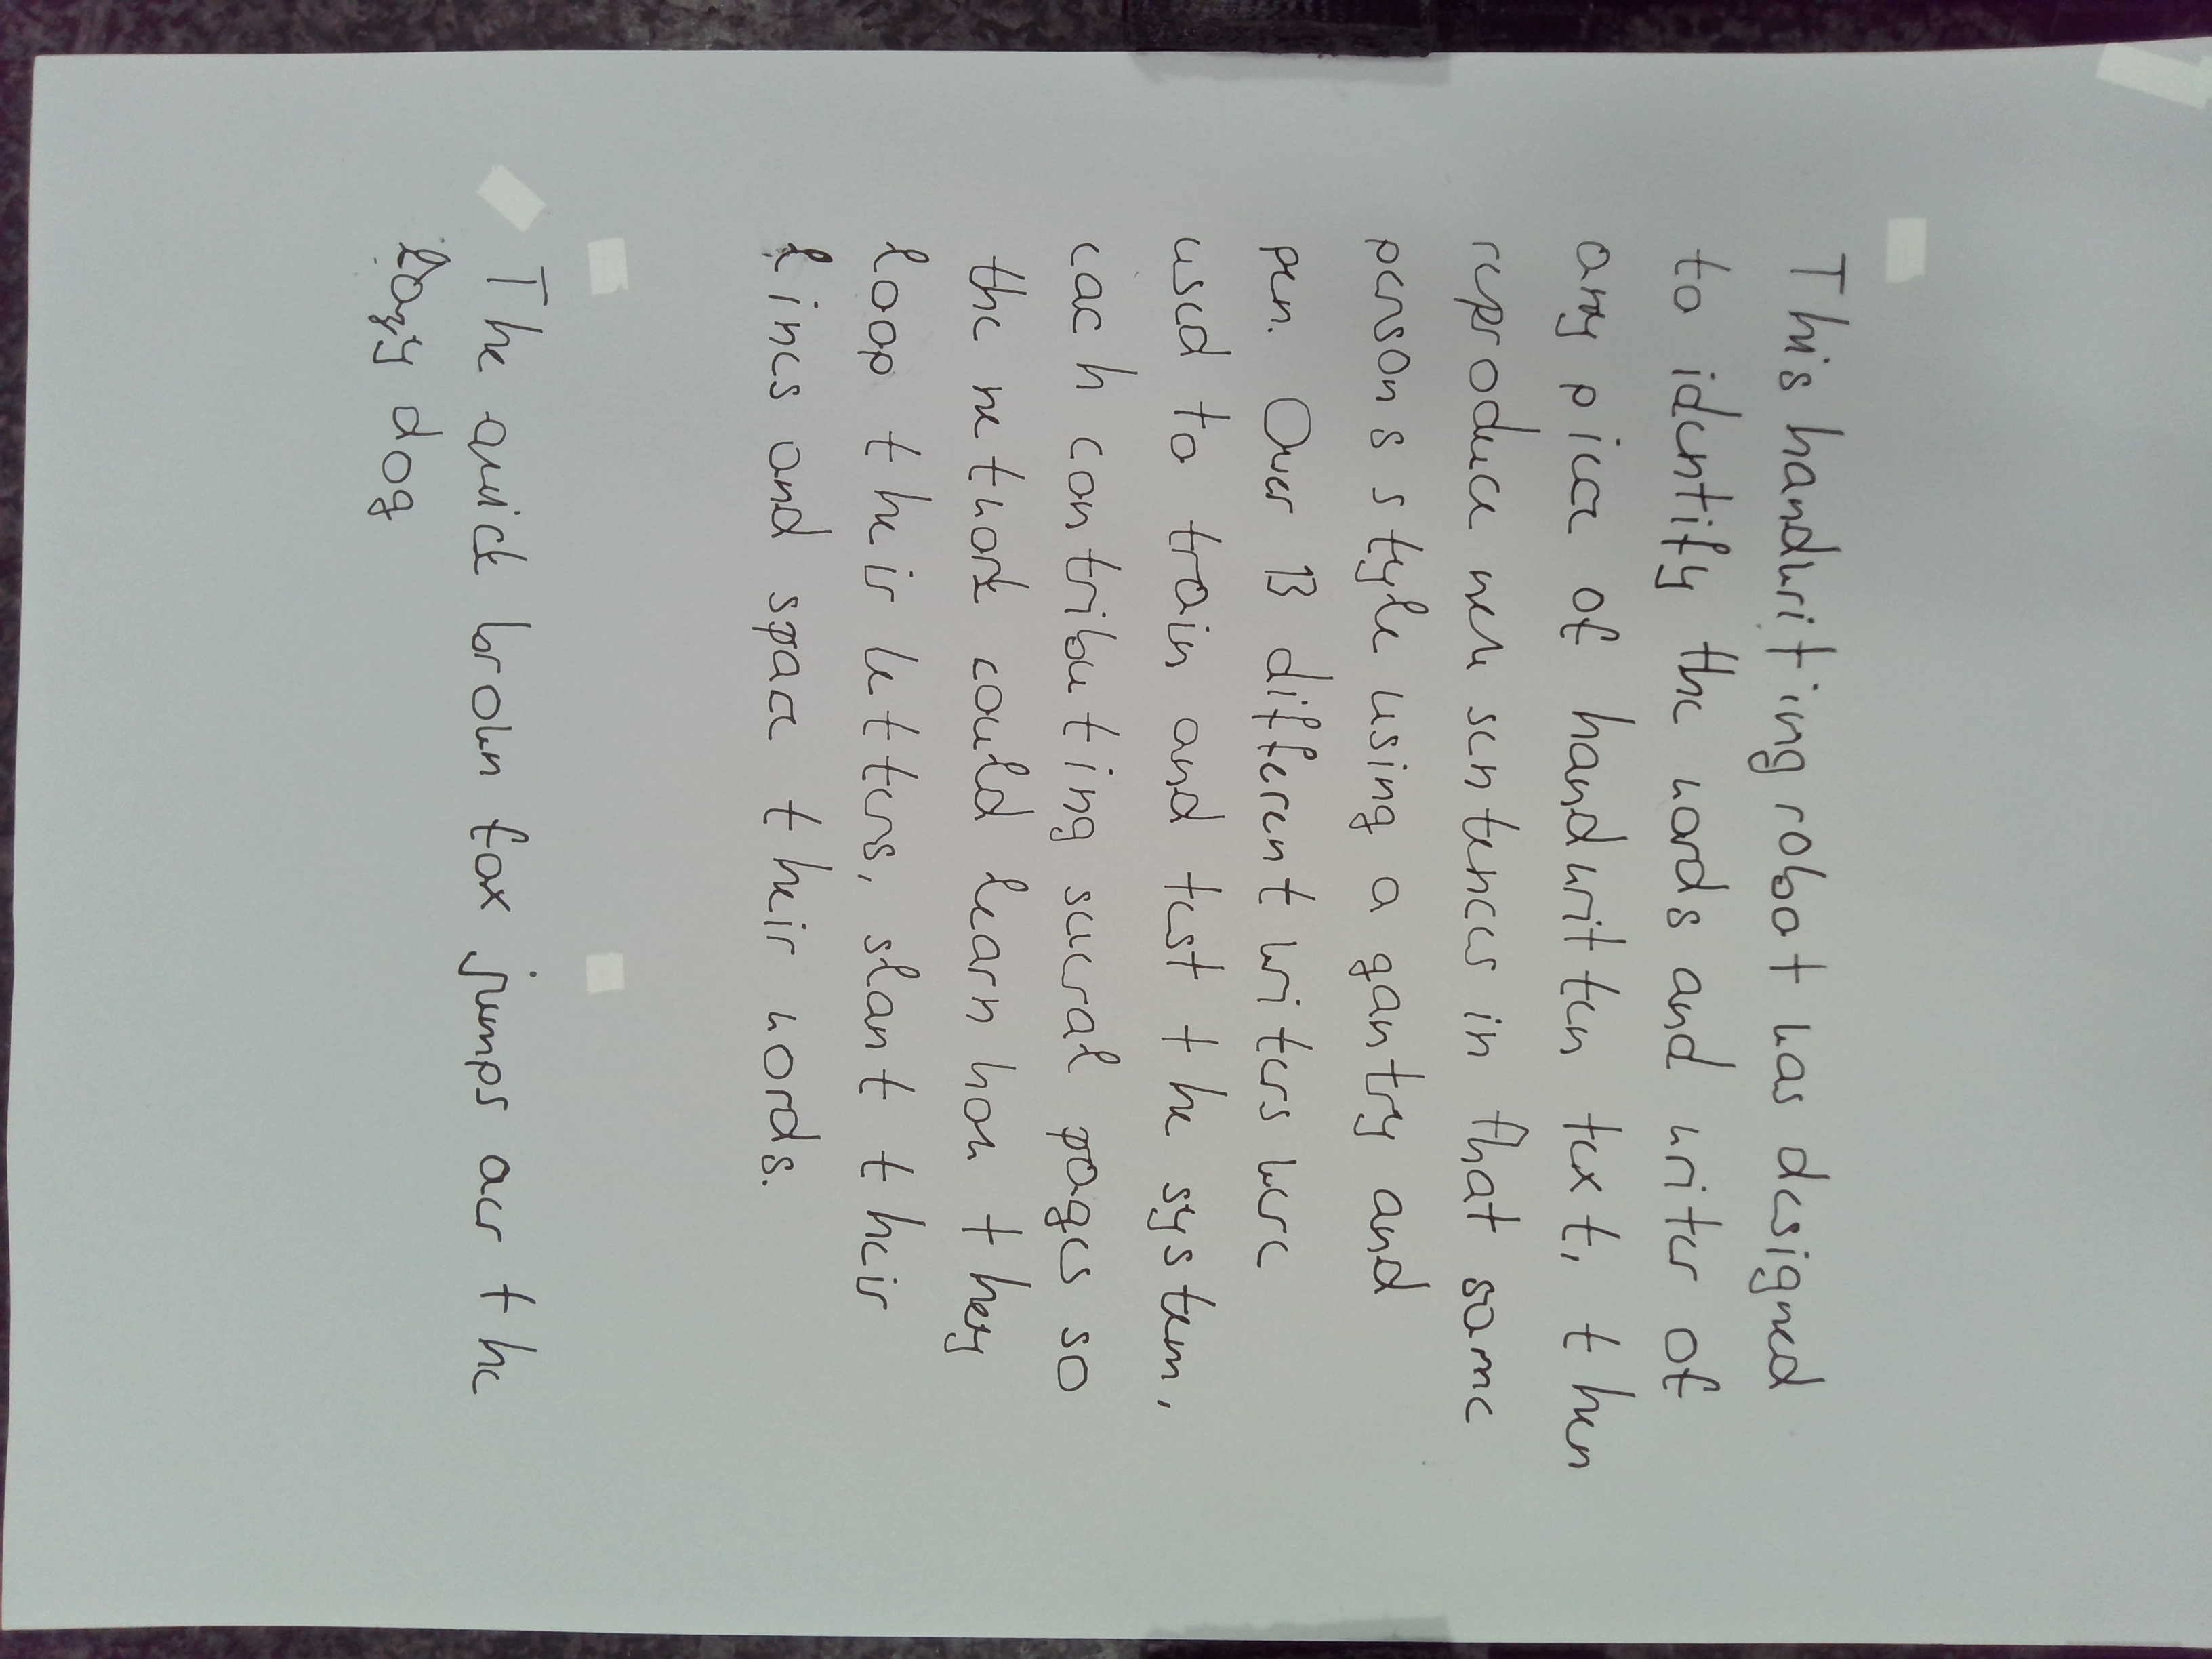
\includegraphics[angle=90,width=\linewidth,height=.55\textheight,keepaspectratio]{Figures/PhysicalPages/Author3841.jpg}\par Author3841\end{minipage}\hfill
\begin{minipage}{.48\linewidth}\centering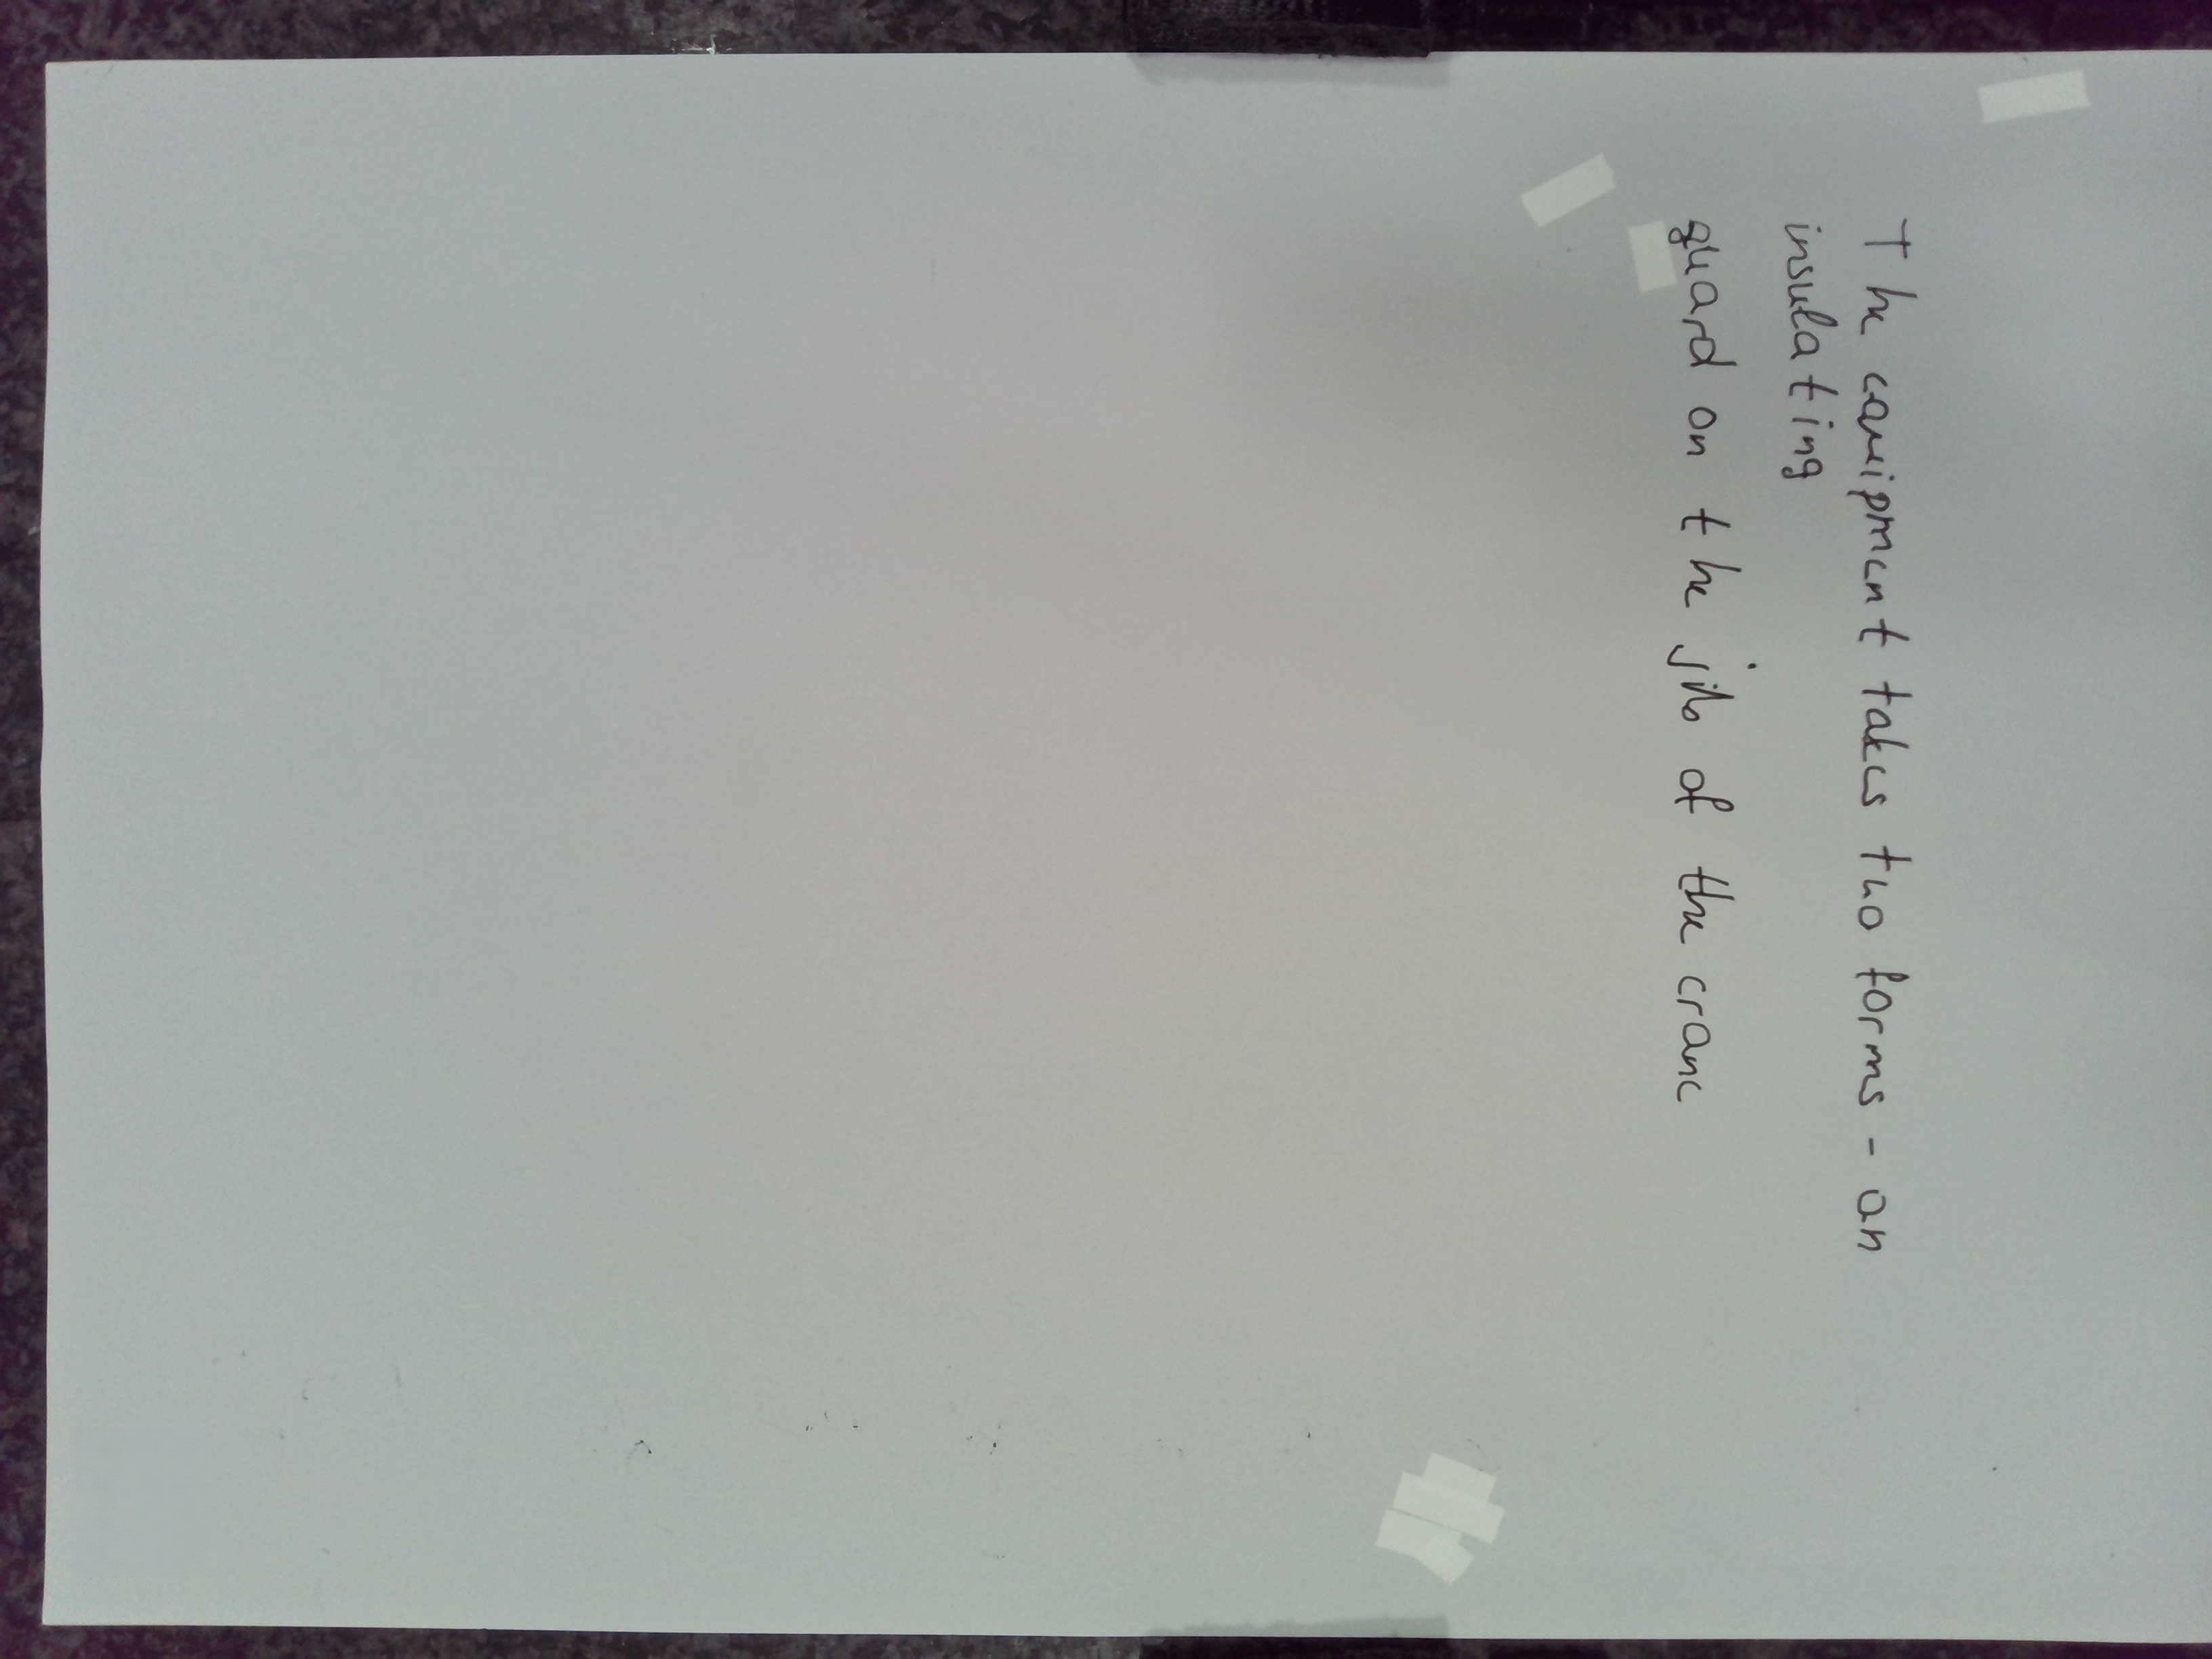
\includegraphics[angle=90,width=\linewidth,height=.55\textheight,keepaspectratio]{Figures/PhysicalPages/Author3842.jpg}\par Author3842\end{minipage}\hfill
\caption{Physical pages Author3841, Author3842.}\label{fig:app-physical-pages-3}\end{figure}
\begin{figure}[!htbp]\centering
\begin{minipage}{.48\linewidth}\centering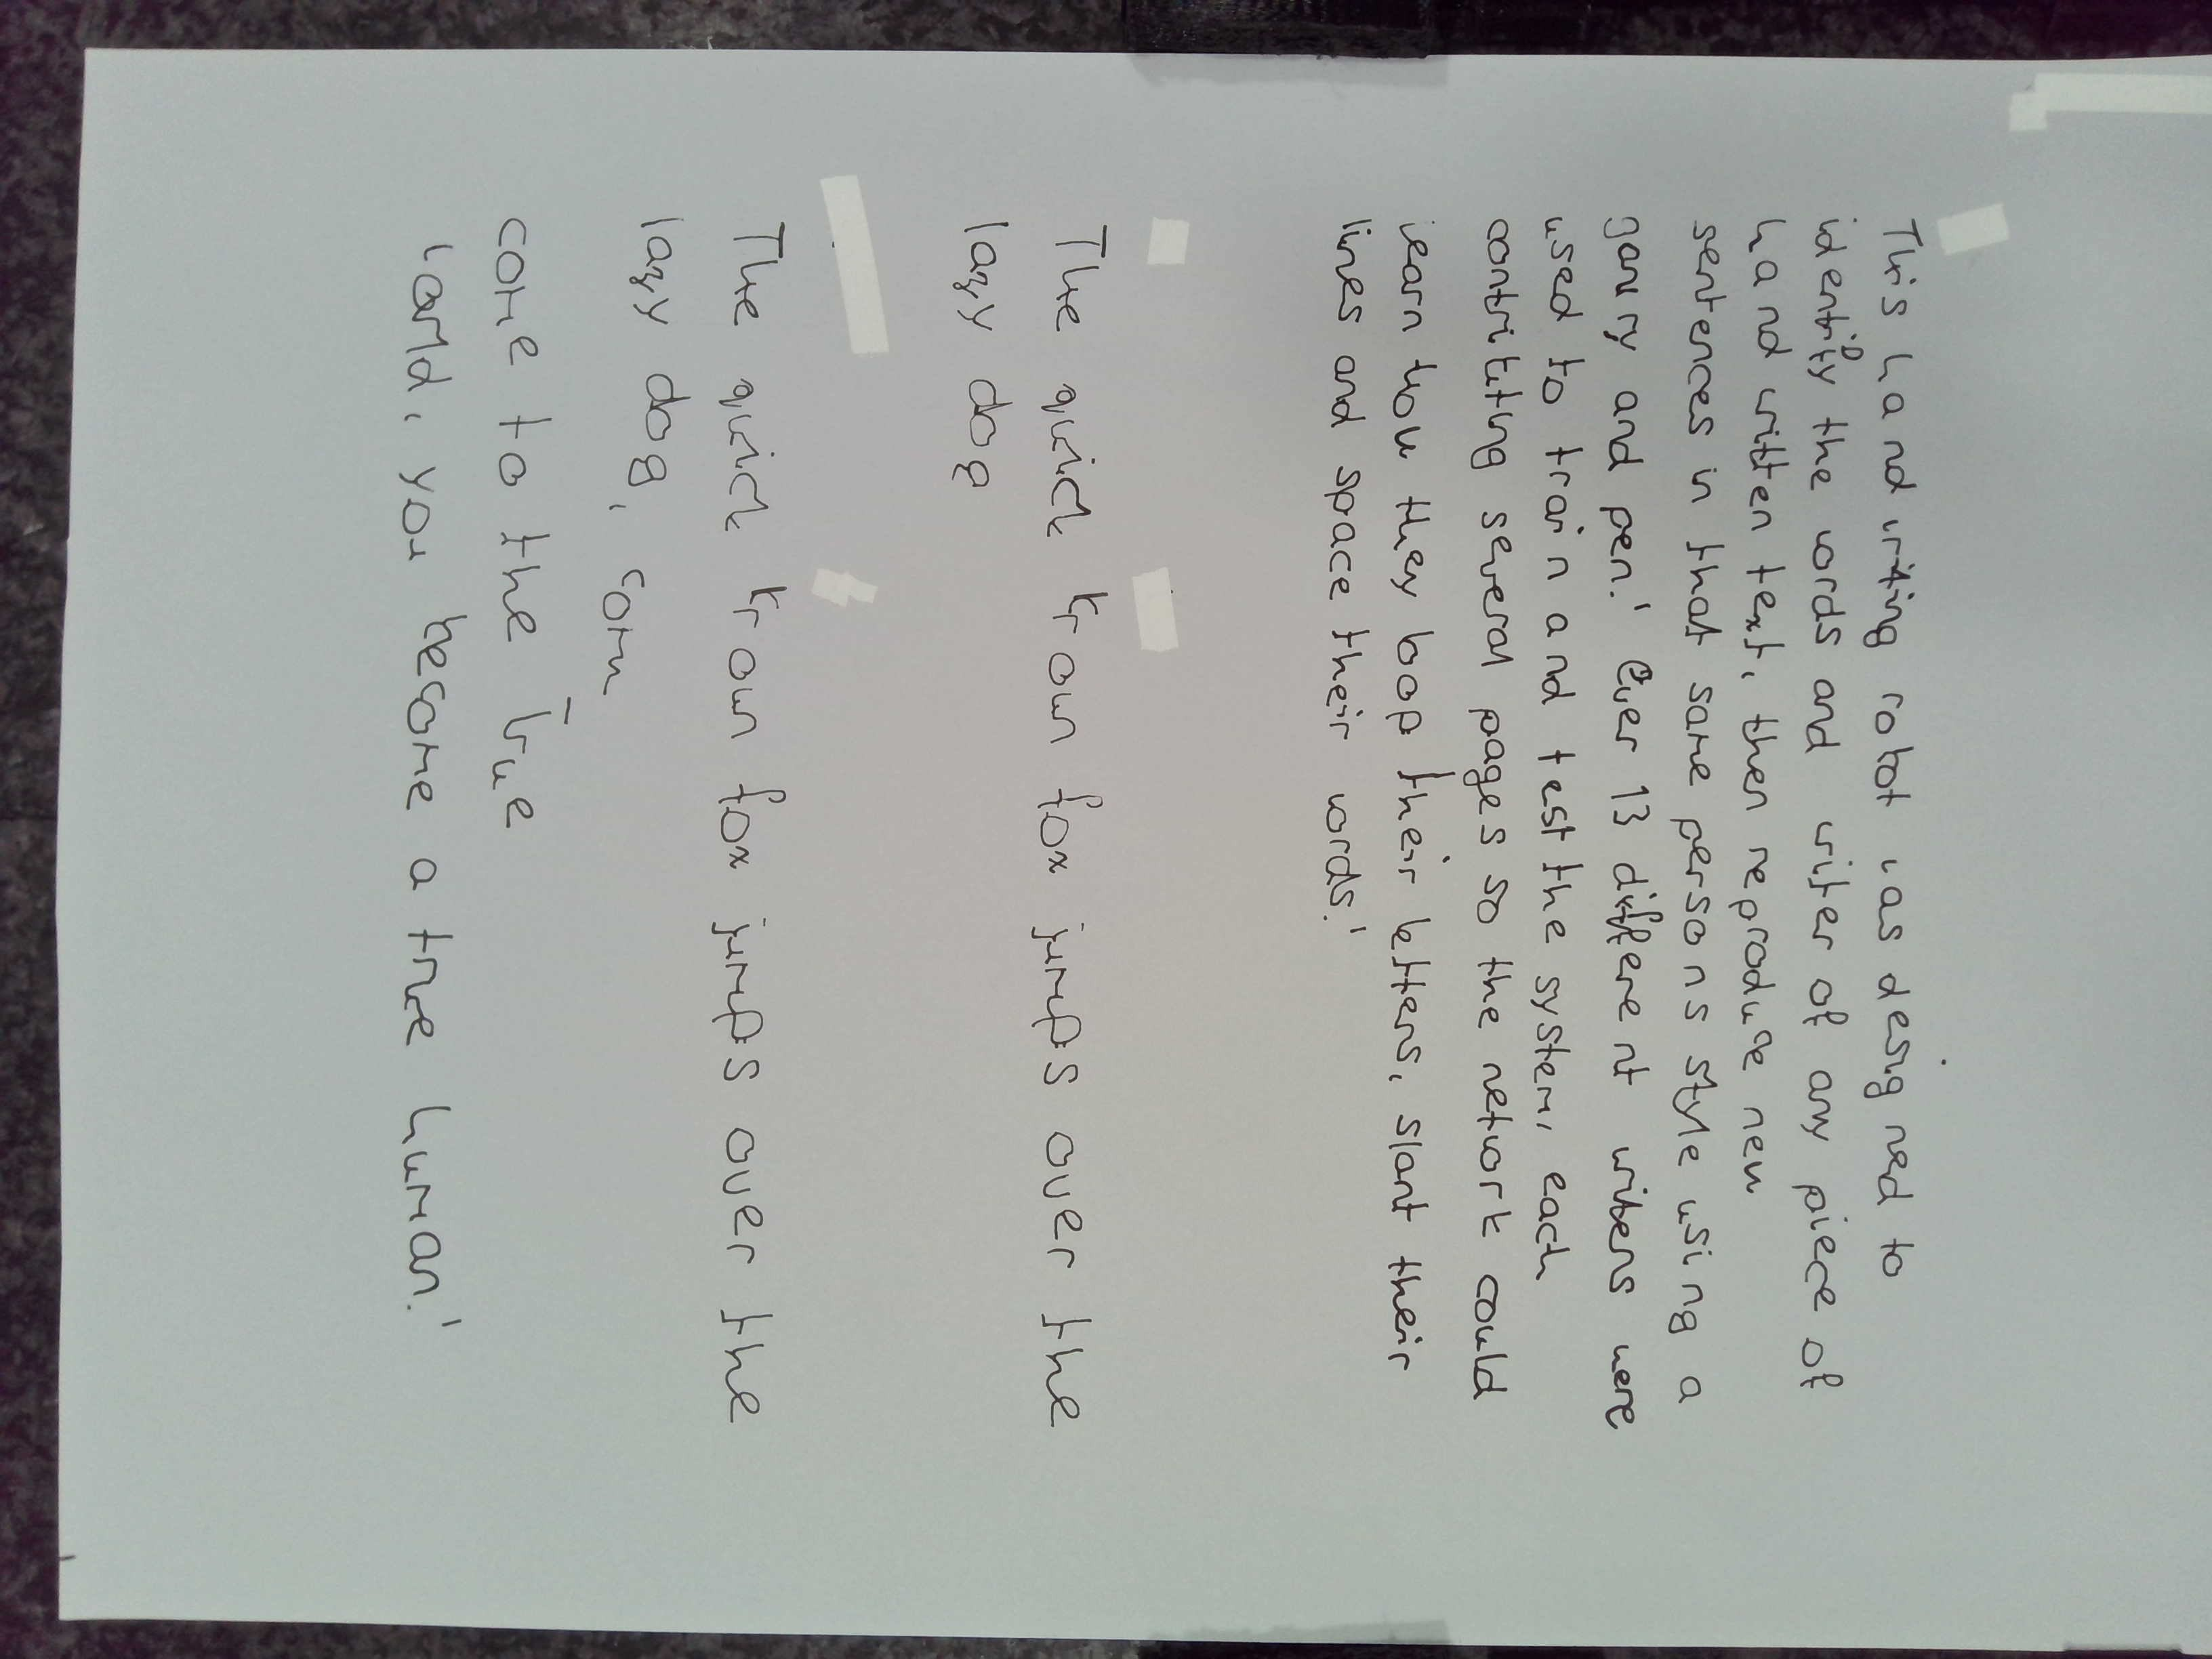
\includegraphics[angle=90,width=\linewidth,height=.55\textheight,keepaspectratio]{Figures/PhysicalPages/Author552.jpg}\par Author552\end{minipage}\hfill
\begin{minipage}{.48\linewidth}\centering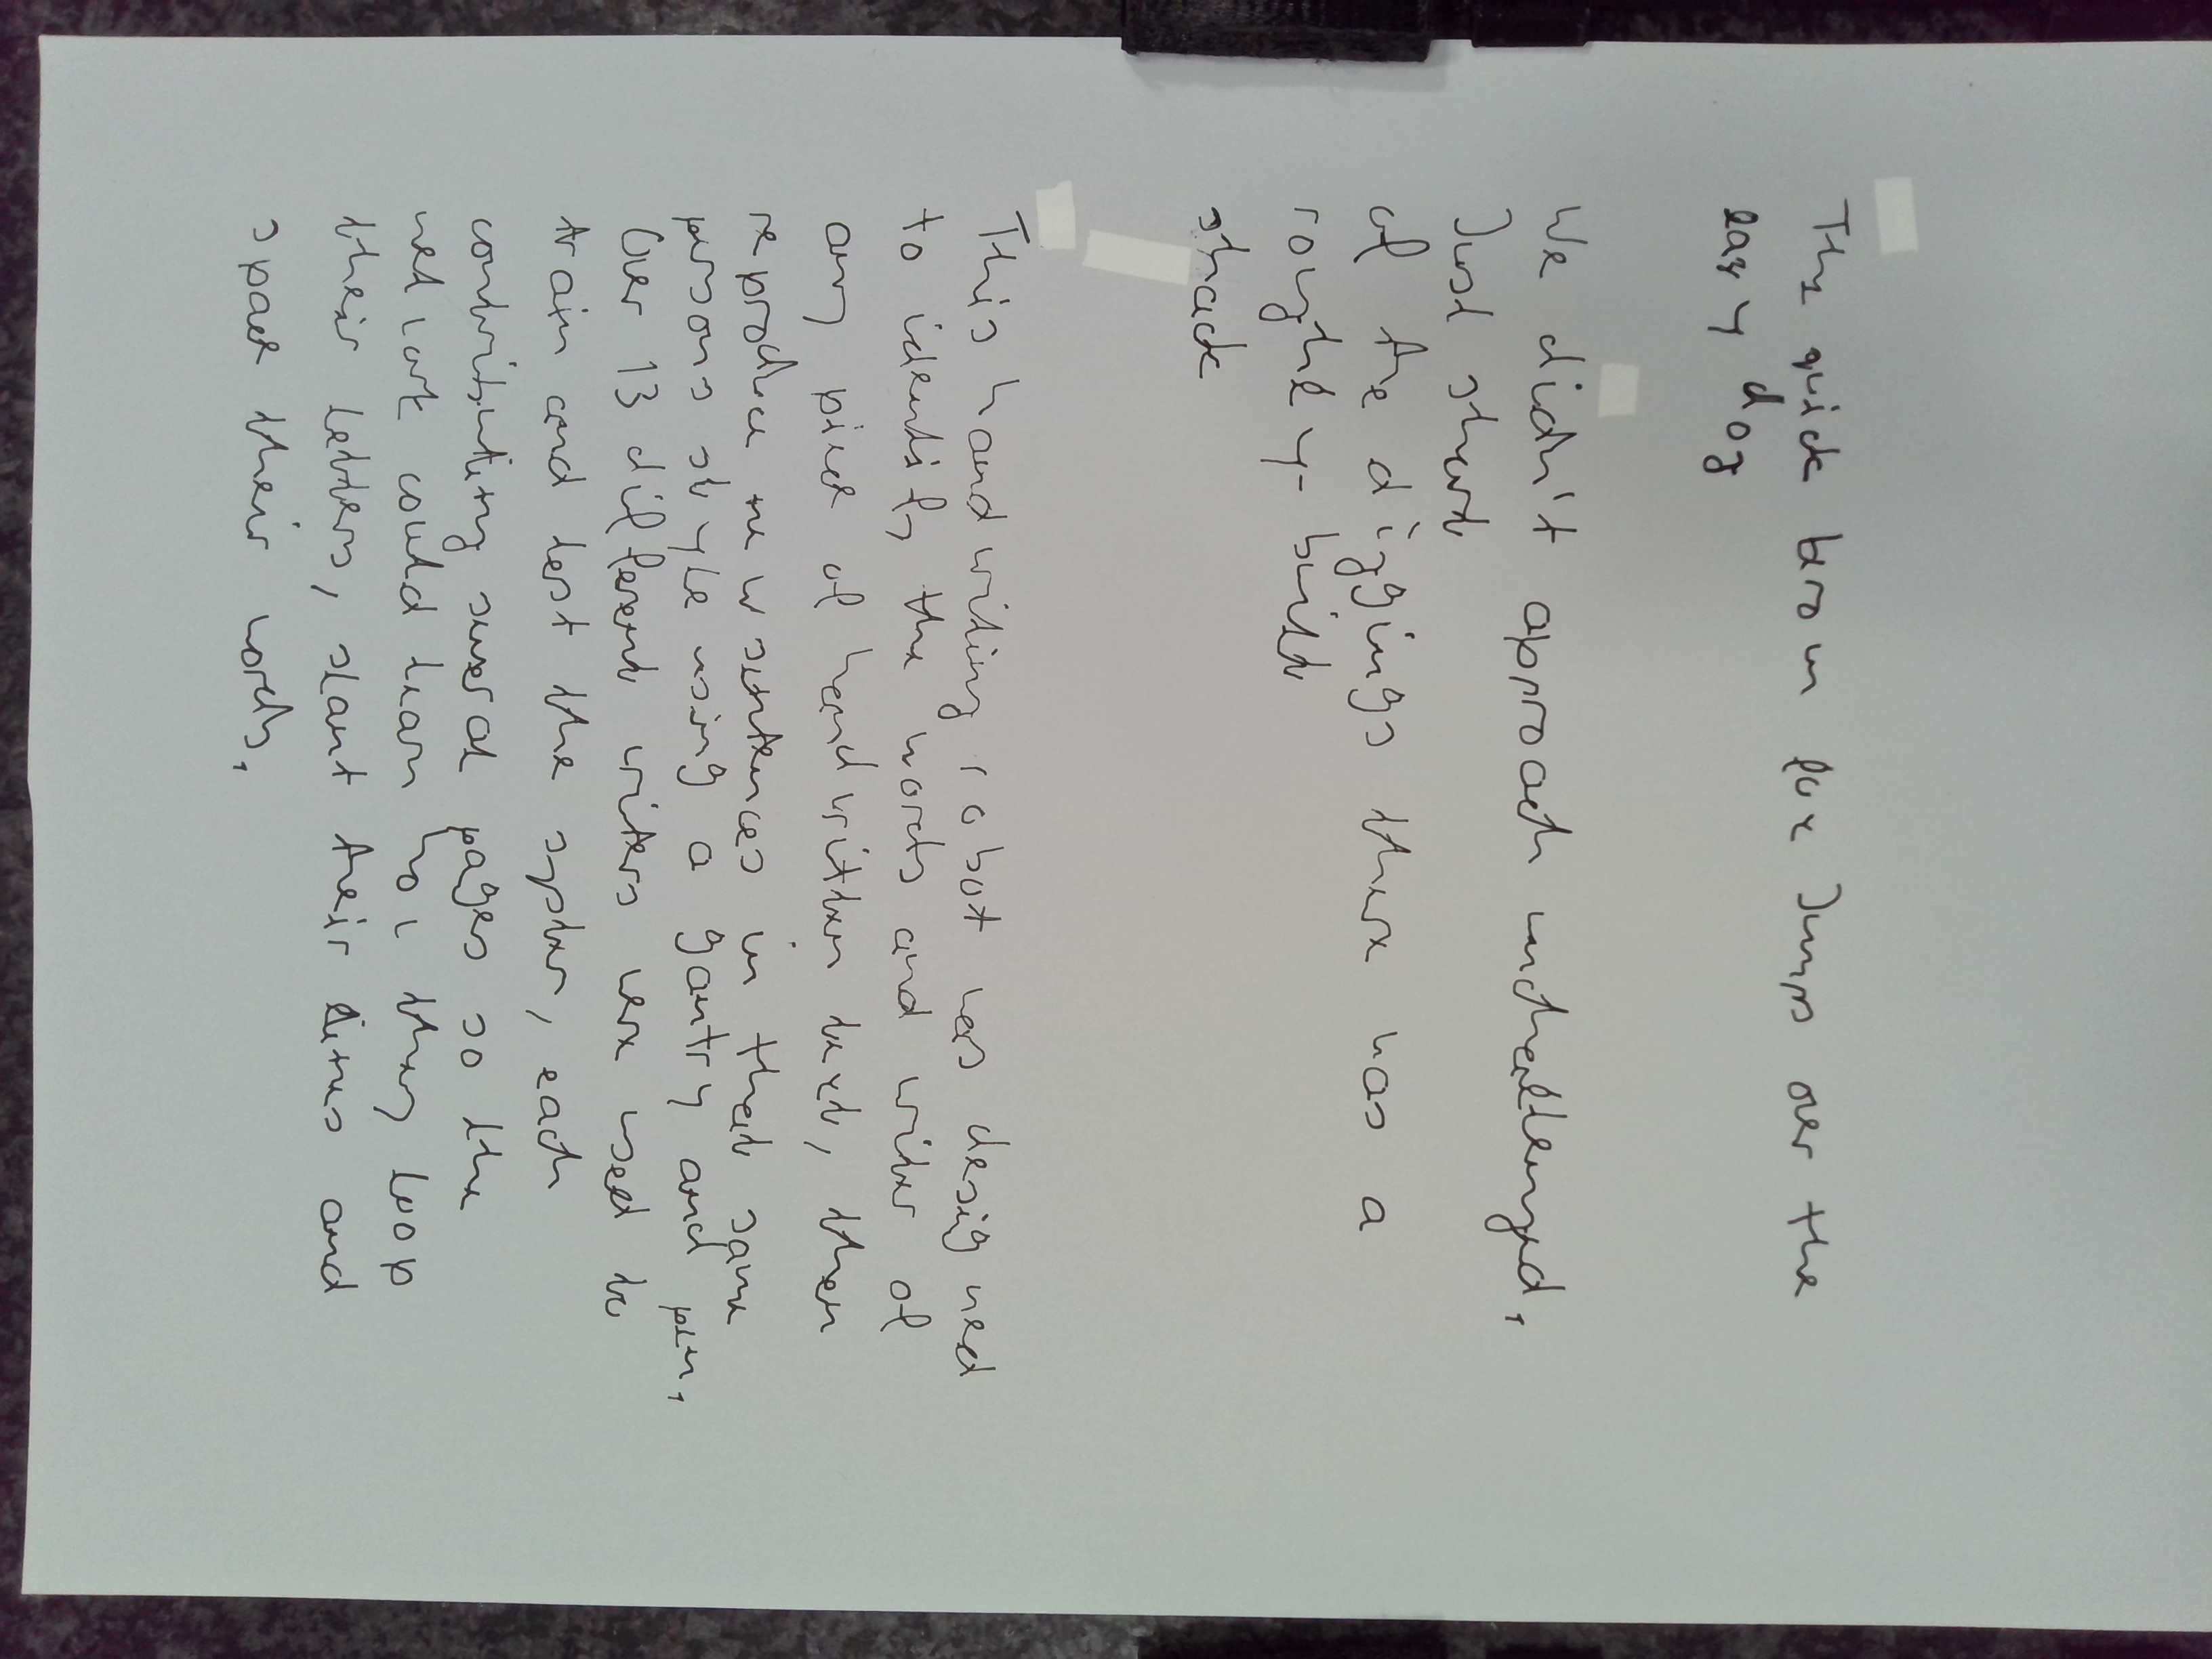
\includegraphics[angle=90,width=\linewidth,height=.55\textheight,keepaspectratio]{Figures/PhysicalPages/Author588.jpg}\par Author588\end{minipage}\hfill
\caption{Physical pages Author552, Author588.}\label{fig:app-physical-pages-4}\end{figure}
\begin{figure}[!htbp]\centering
\begin{minipage}{.48\linewidth}\centering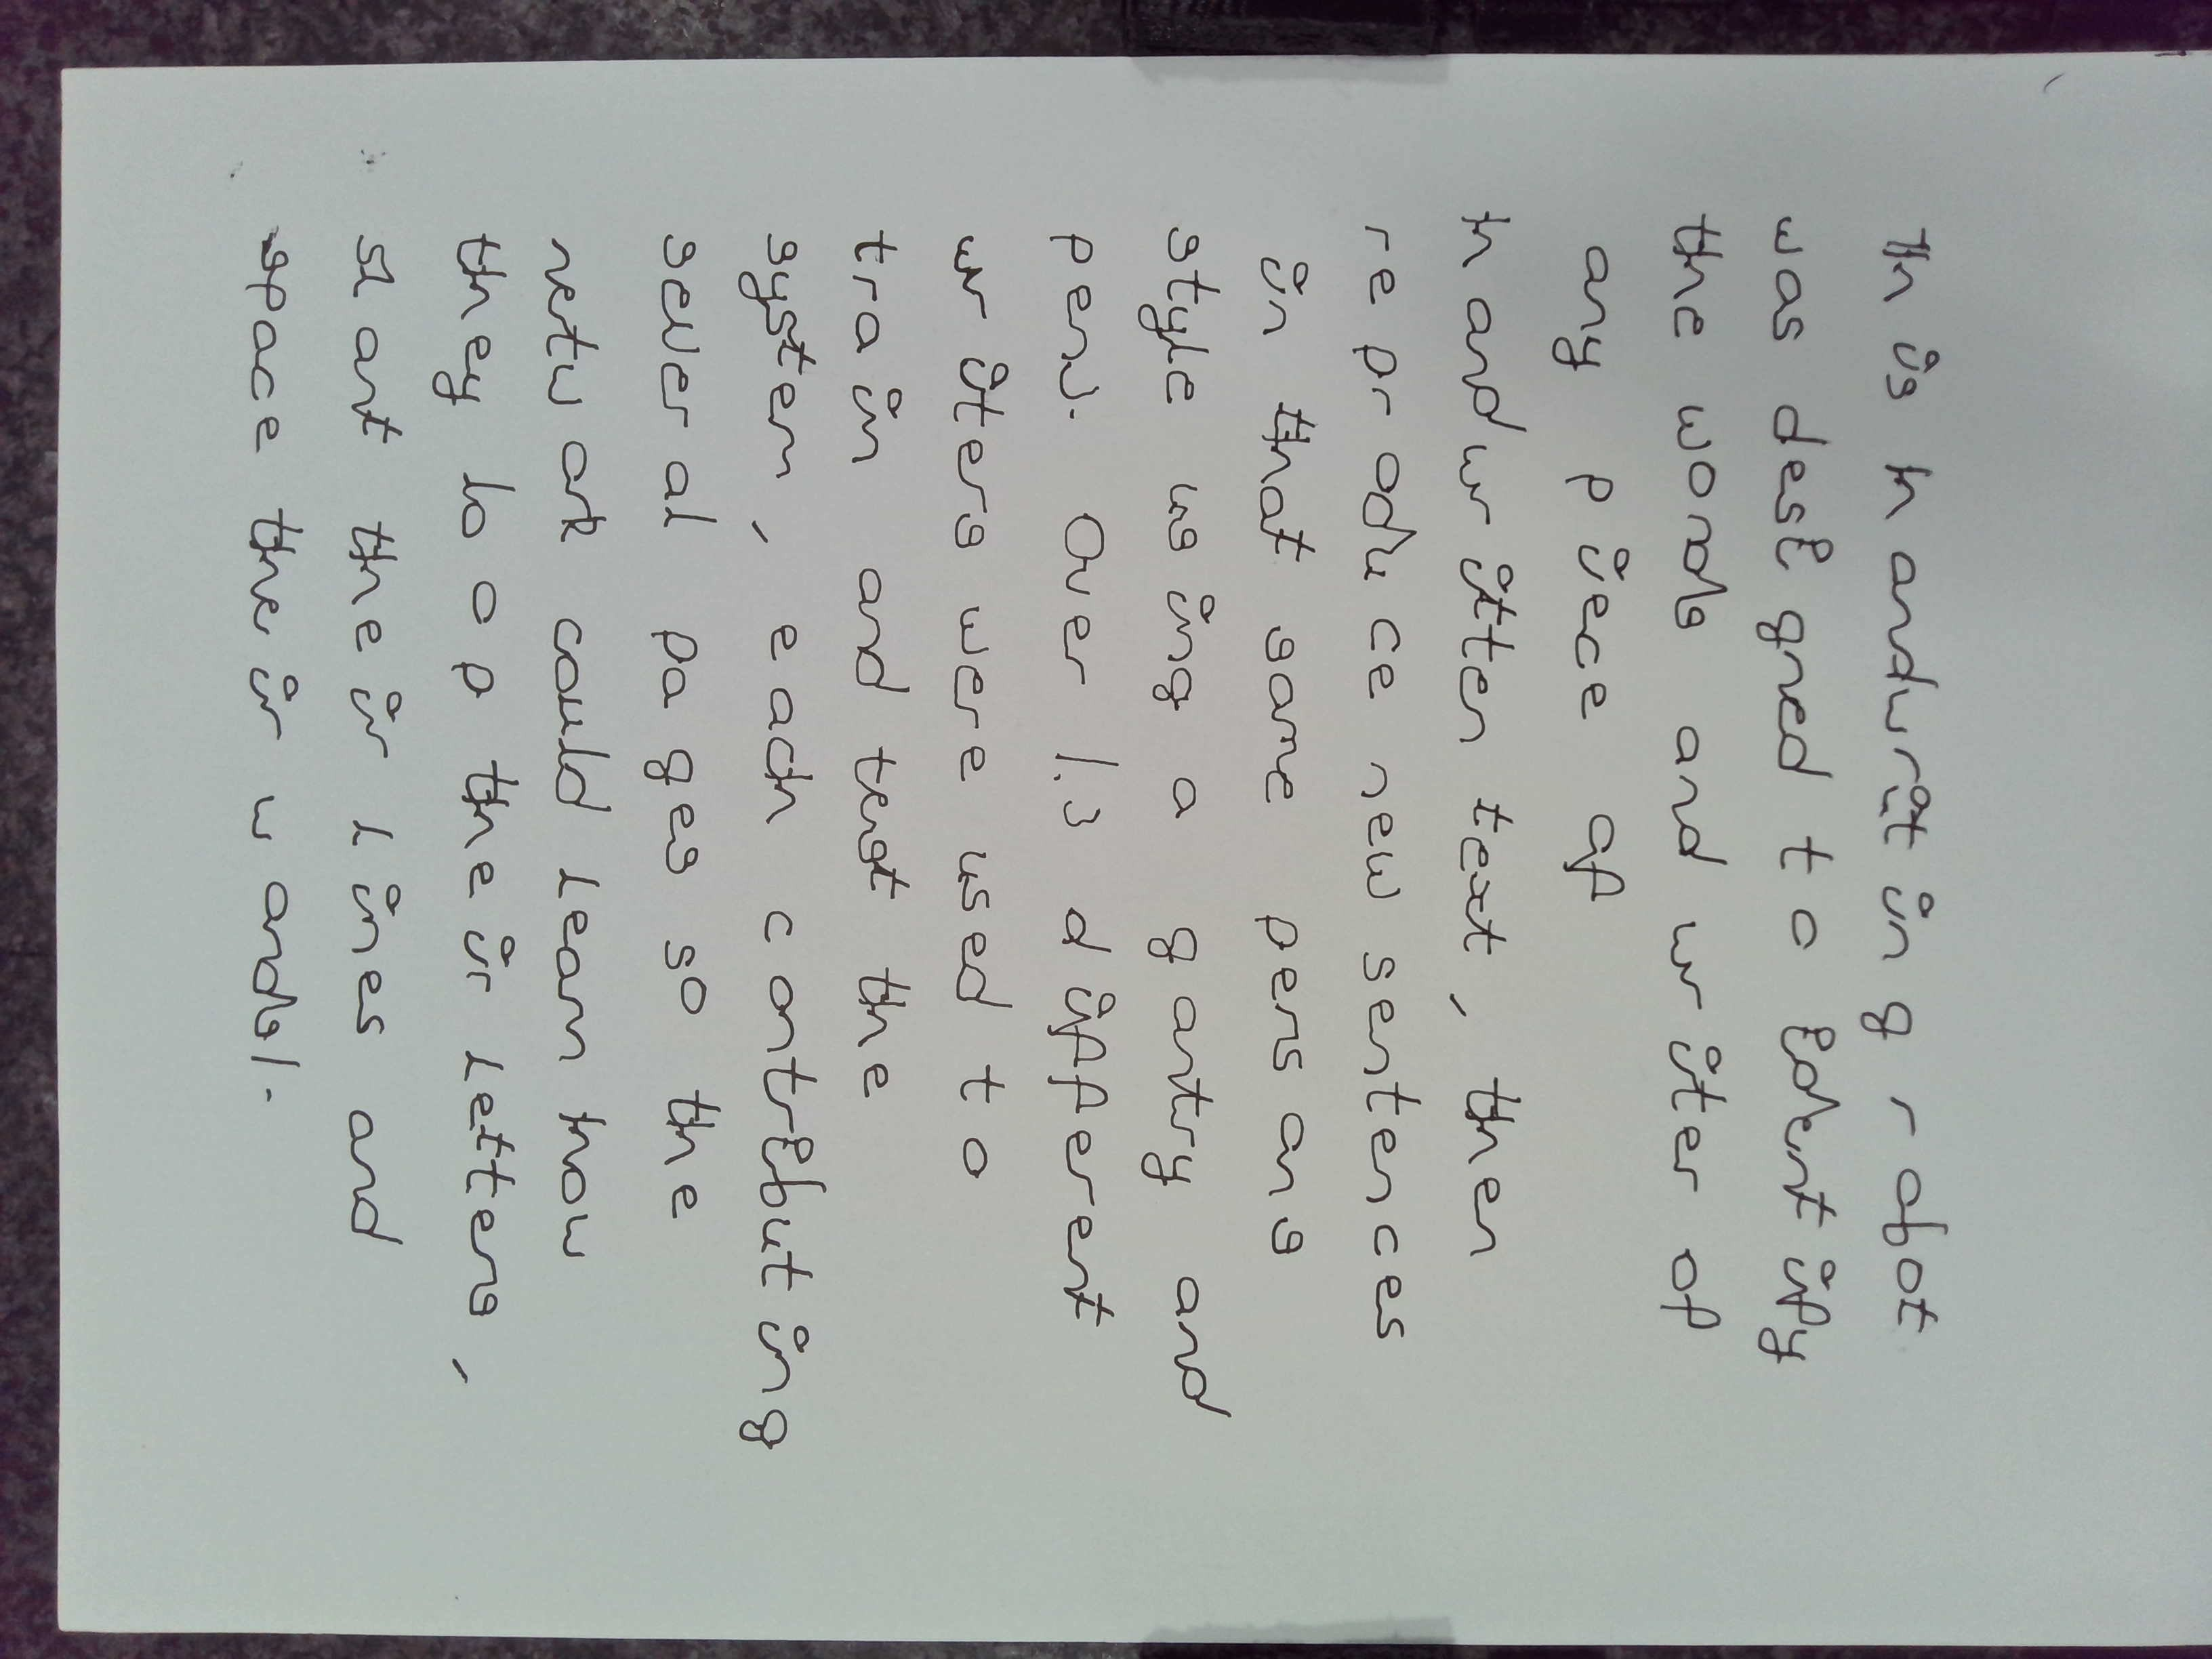
\includegraphics[angle=90,width=\linewidth,height=.55\textheight,keepaspectratio]{Figures/PhysicalPages/AuthorA1.jpg}\par AuthorA1\end{minipage}\hfill
\begin{minipage}{.48\linewidth}\centering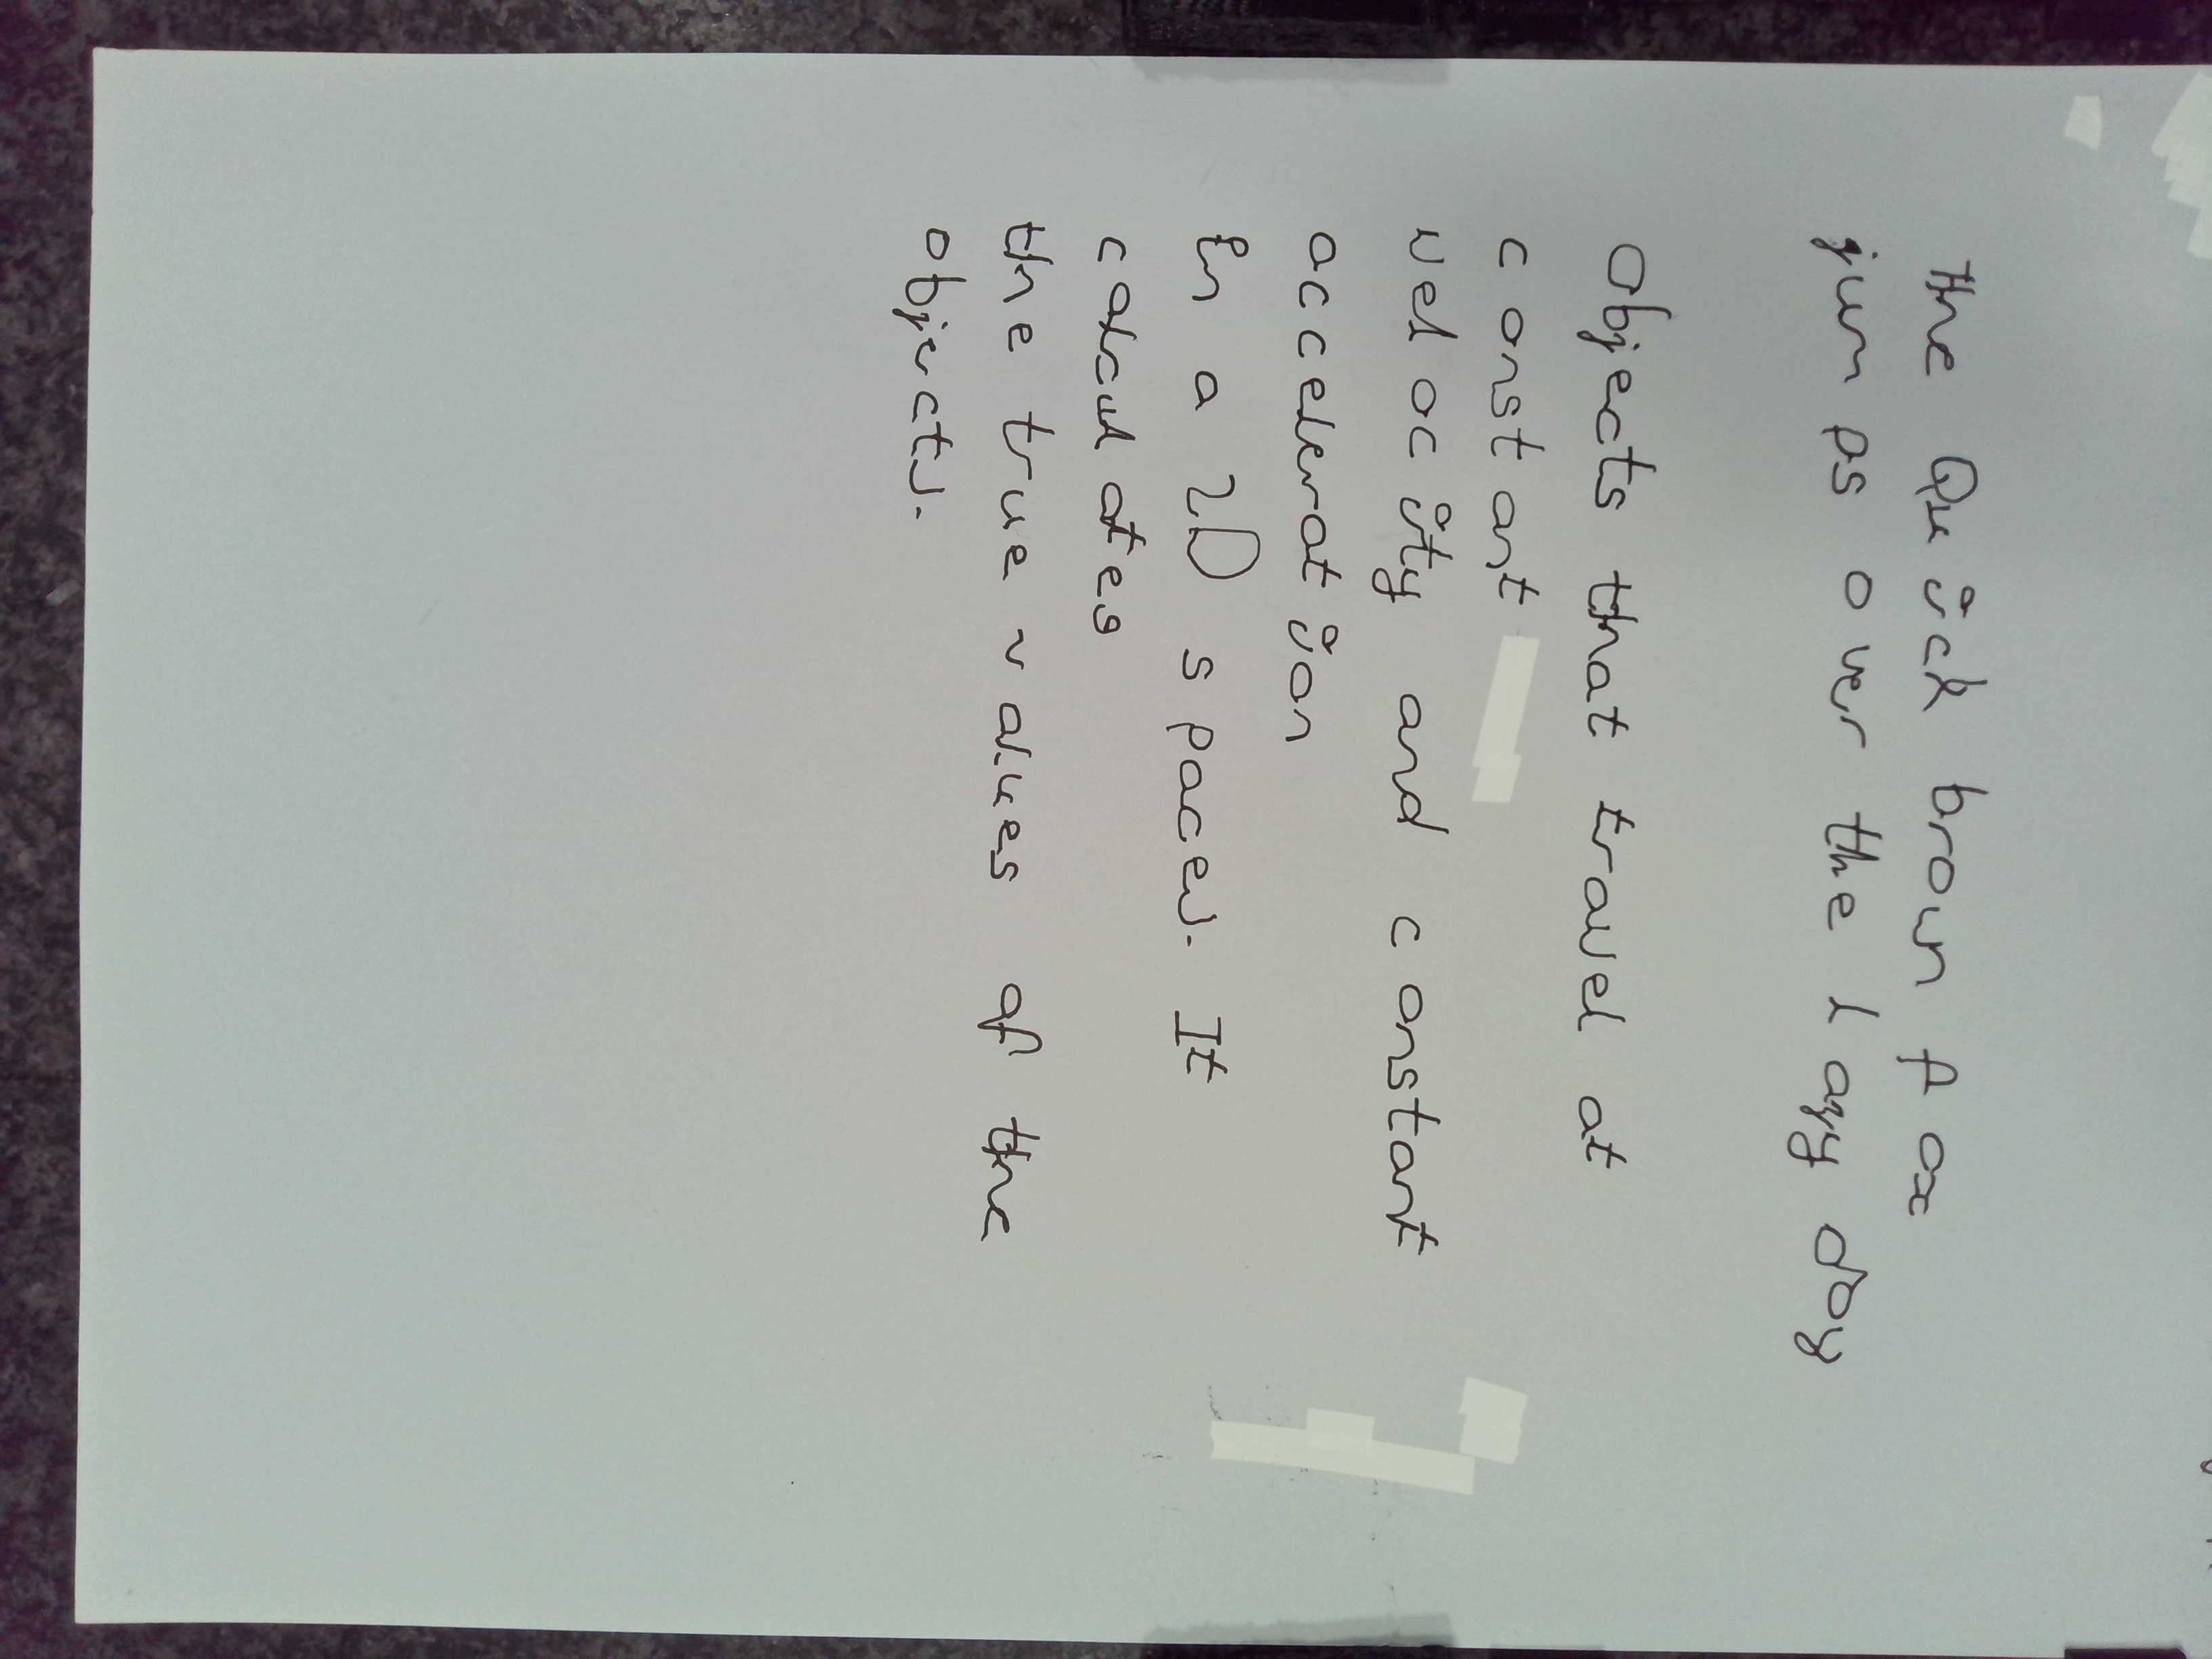
\includegraphics[angle=90,width=\linewidth,height=.55\textheight,keepaspectratio]{Figures/PhysicalPages/AuthorA2.jpg}\par AuthorA2\end{minipage}\hfill
\caption{Physical pages AuthorA1, AuthorA2.}\label{fig:app-physical-pages-5}\end{figure}
\begin{figure}[!htbp]\centering
\begin{minipage}{.48\linewidth}\centering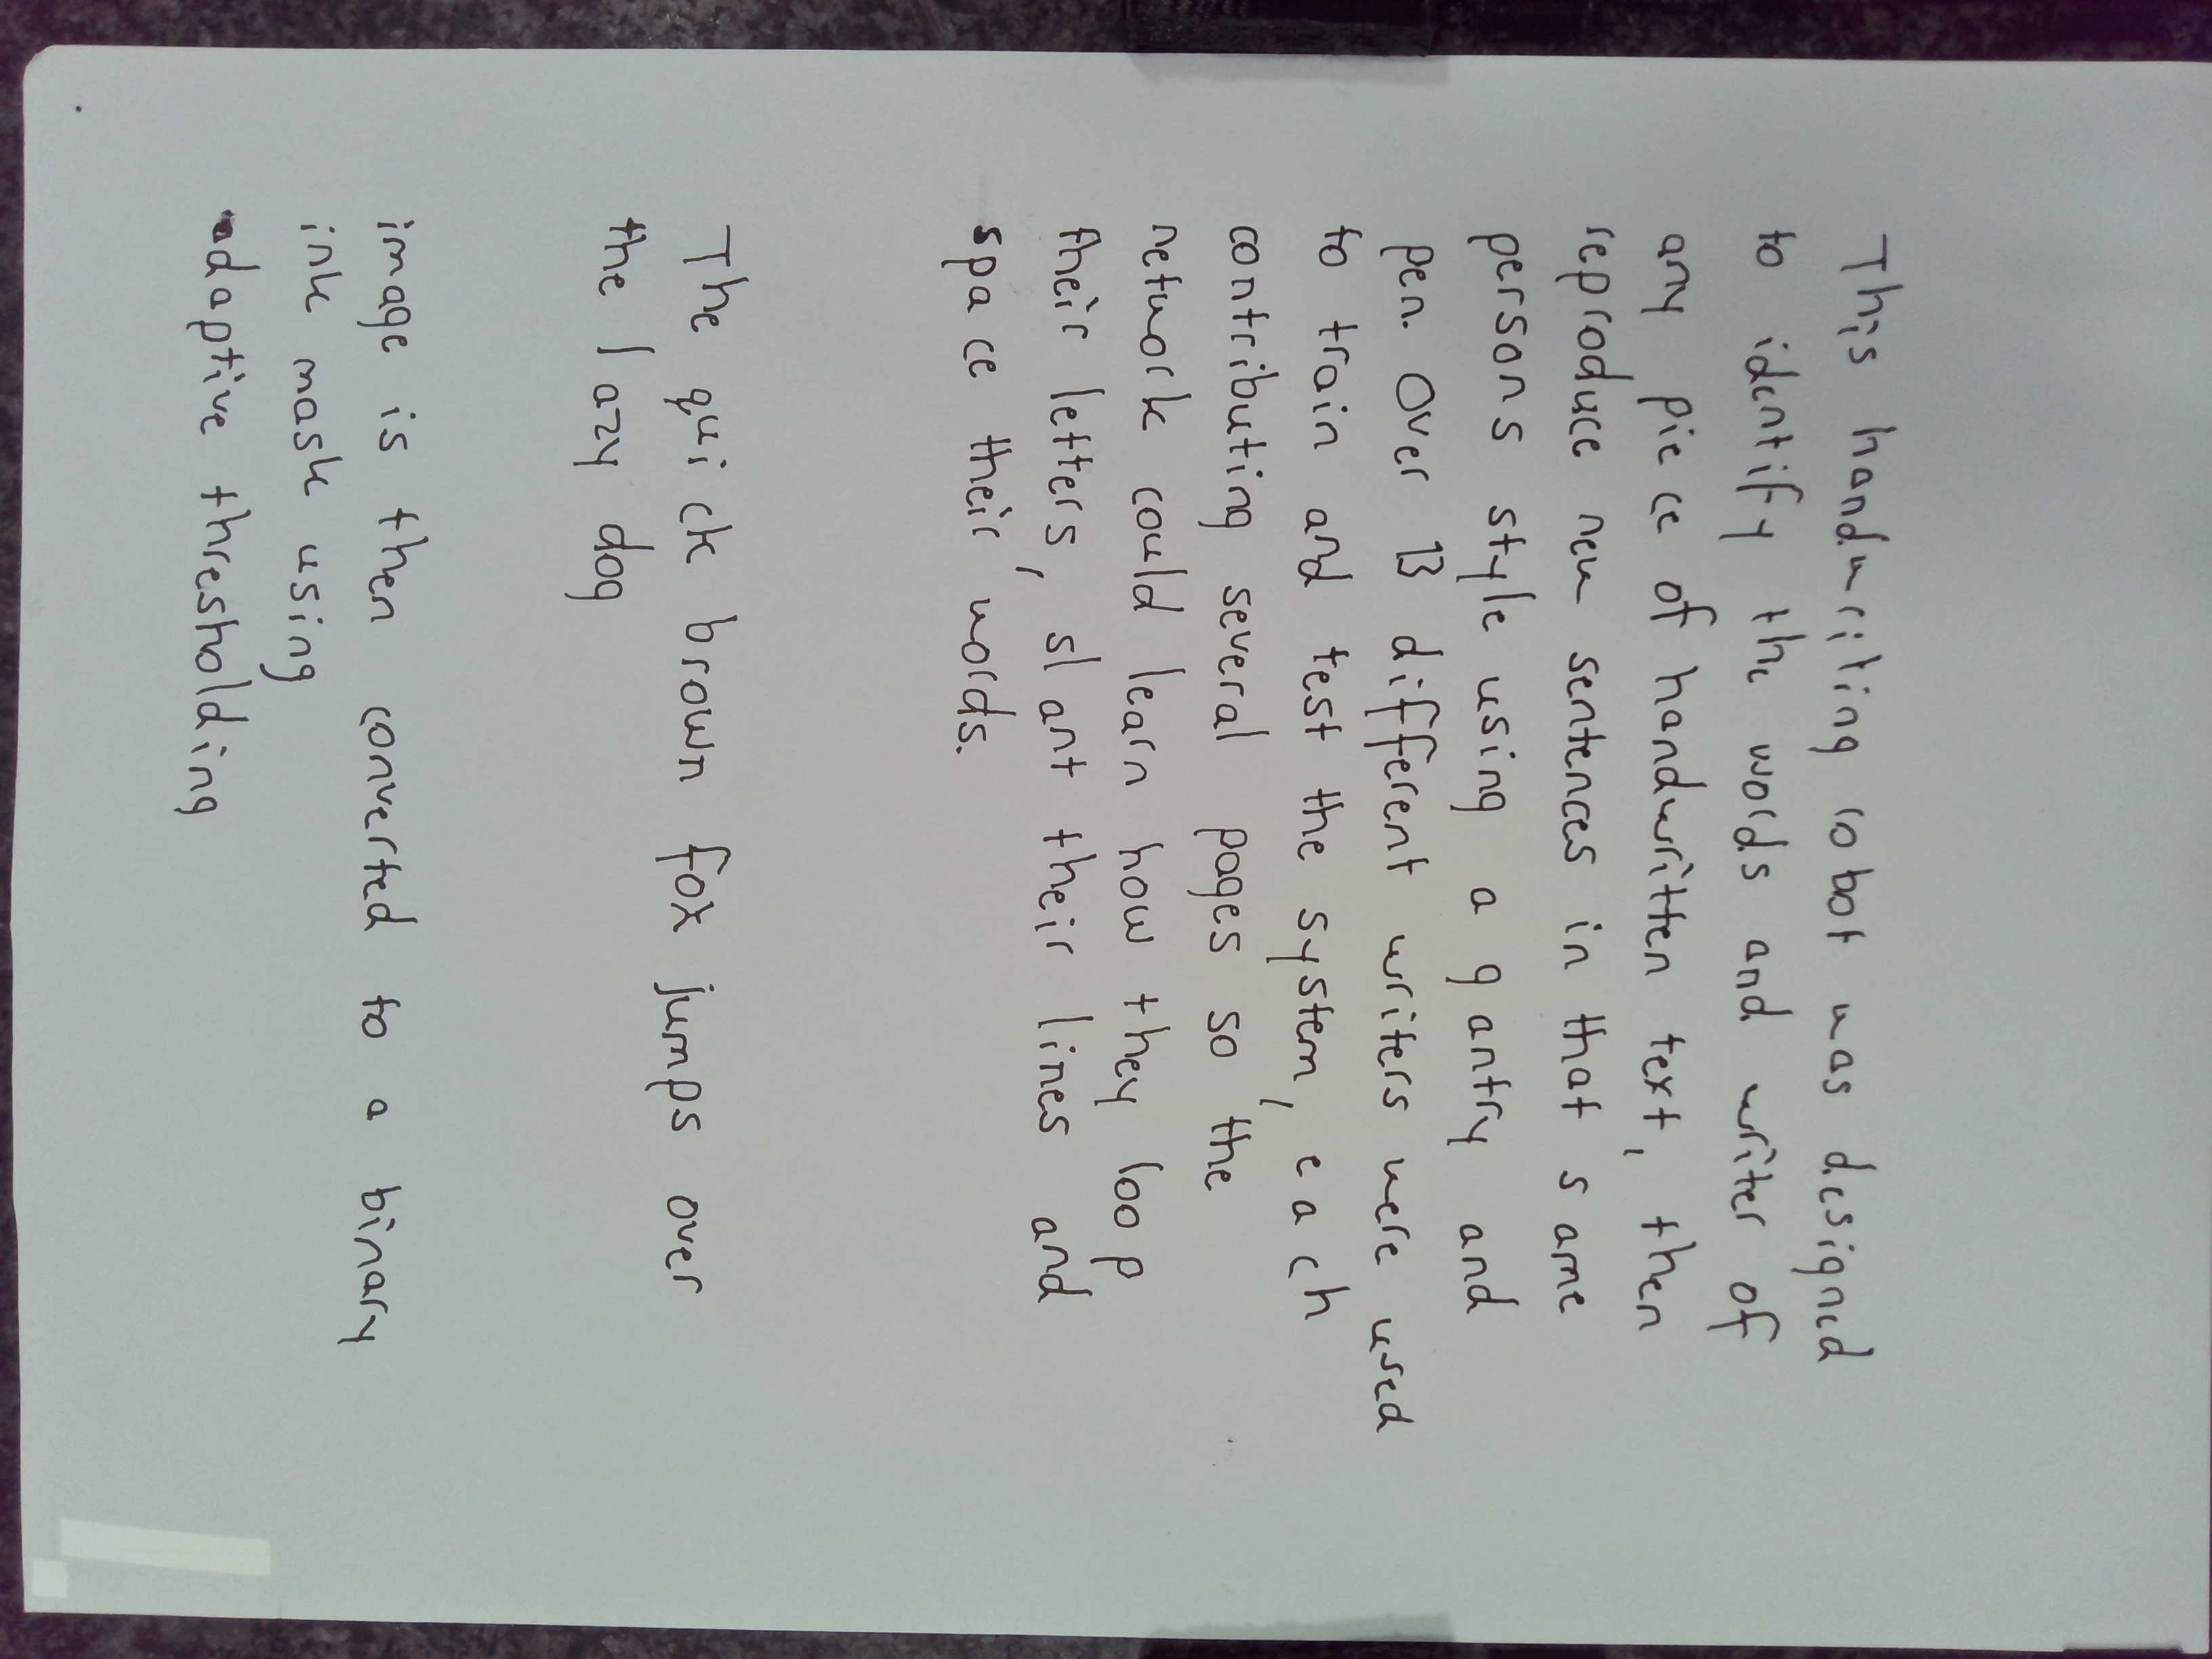
\includegraphics[angle=90,width=\linewidth,height=.55\textheight,keepaspectratio]{Figures/PhysicalPages/AuthorD.jpg}\par AuthorD\end{minipage}\hfill
\begin{minipage}{.48\linewidth}\centering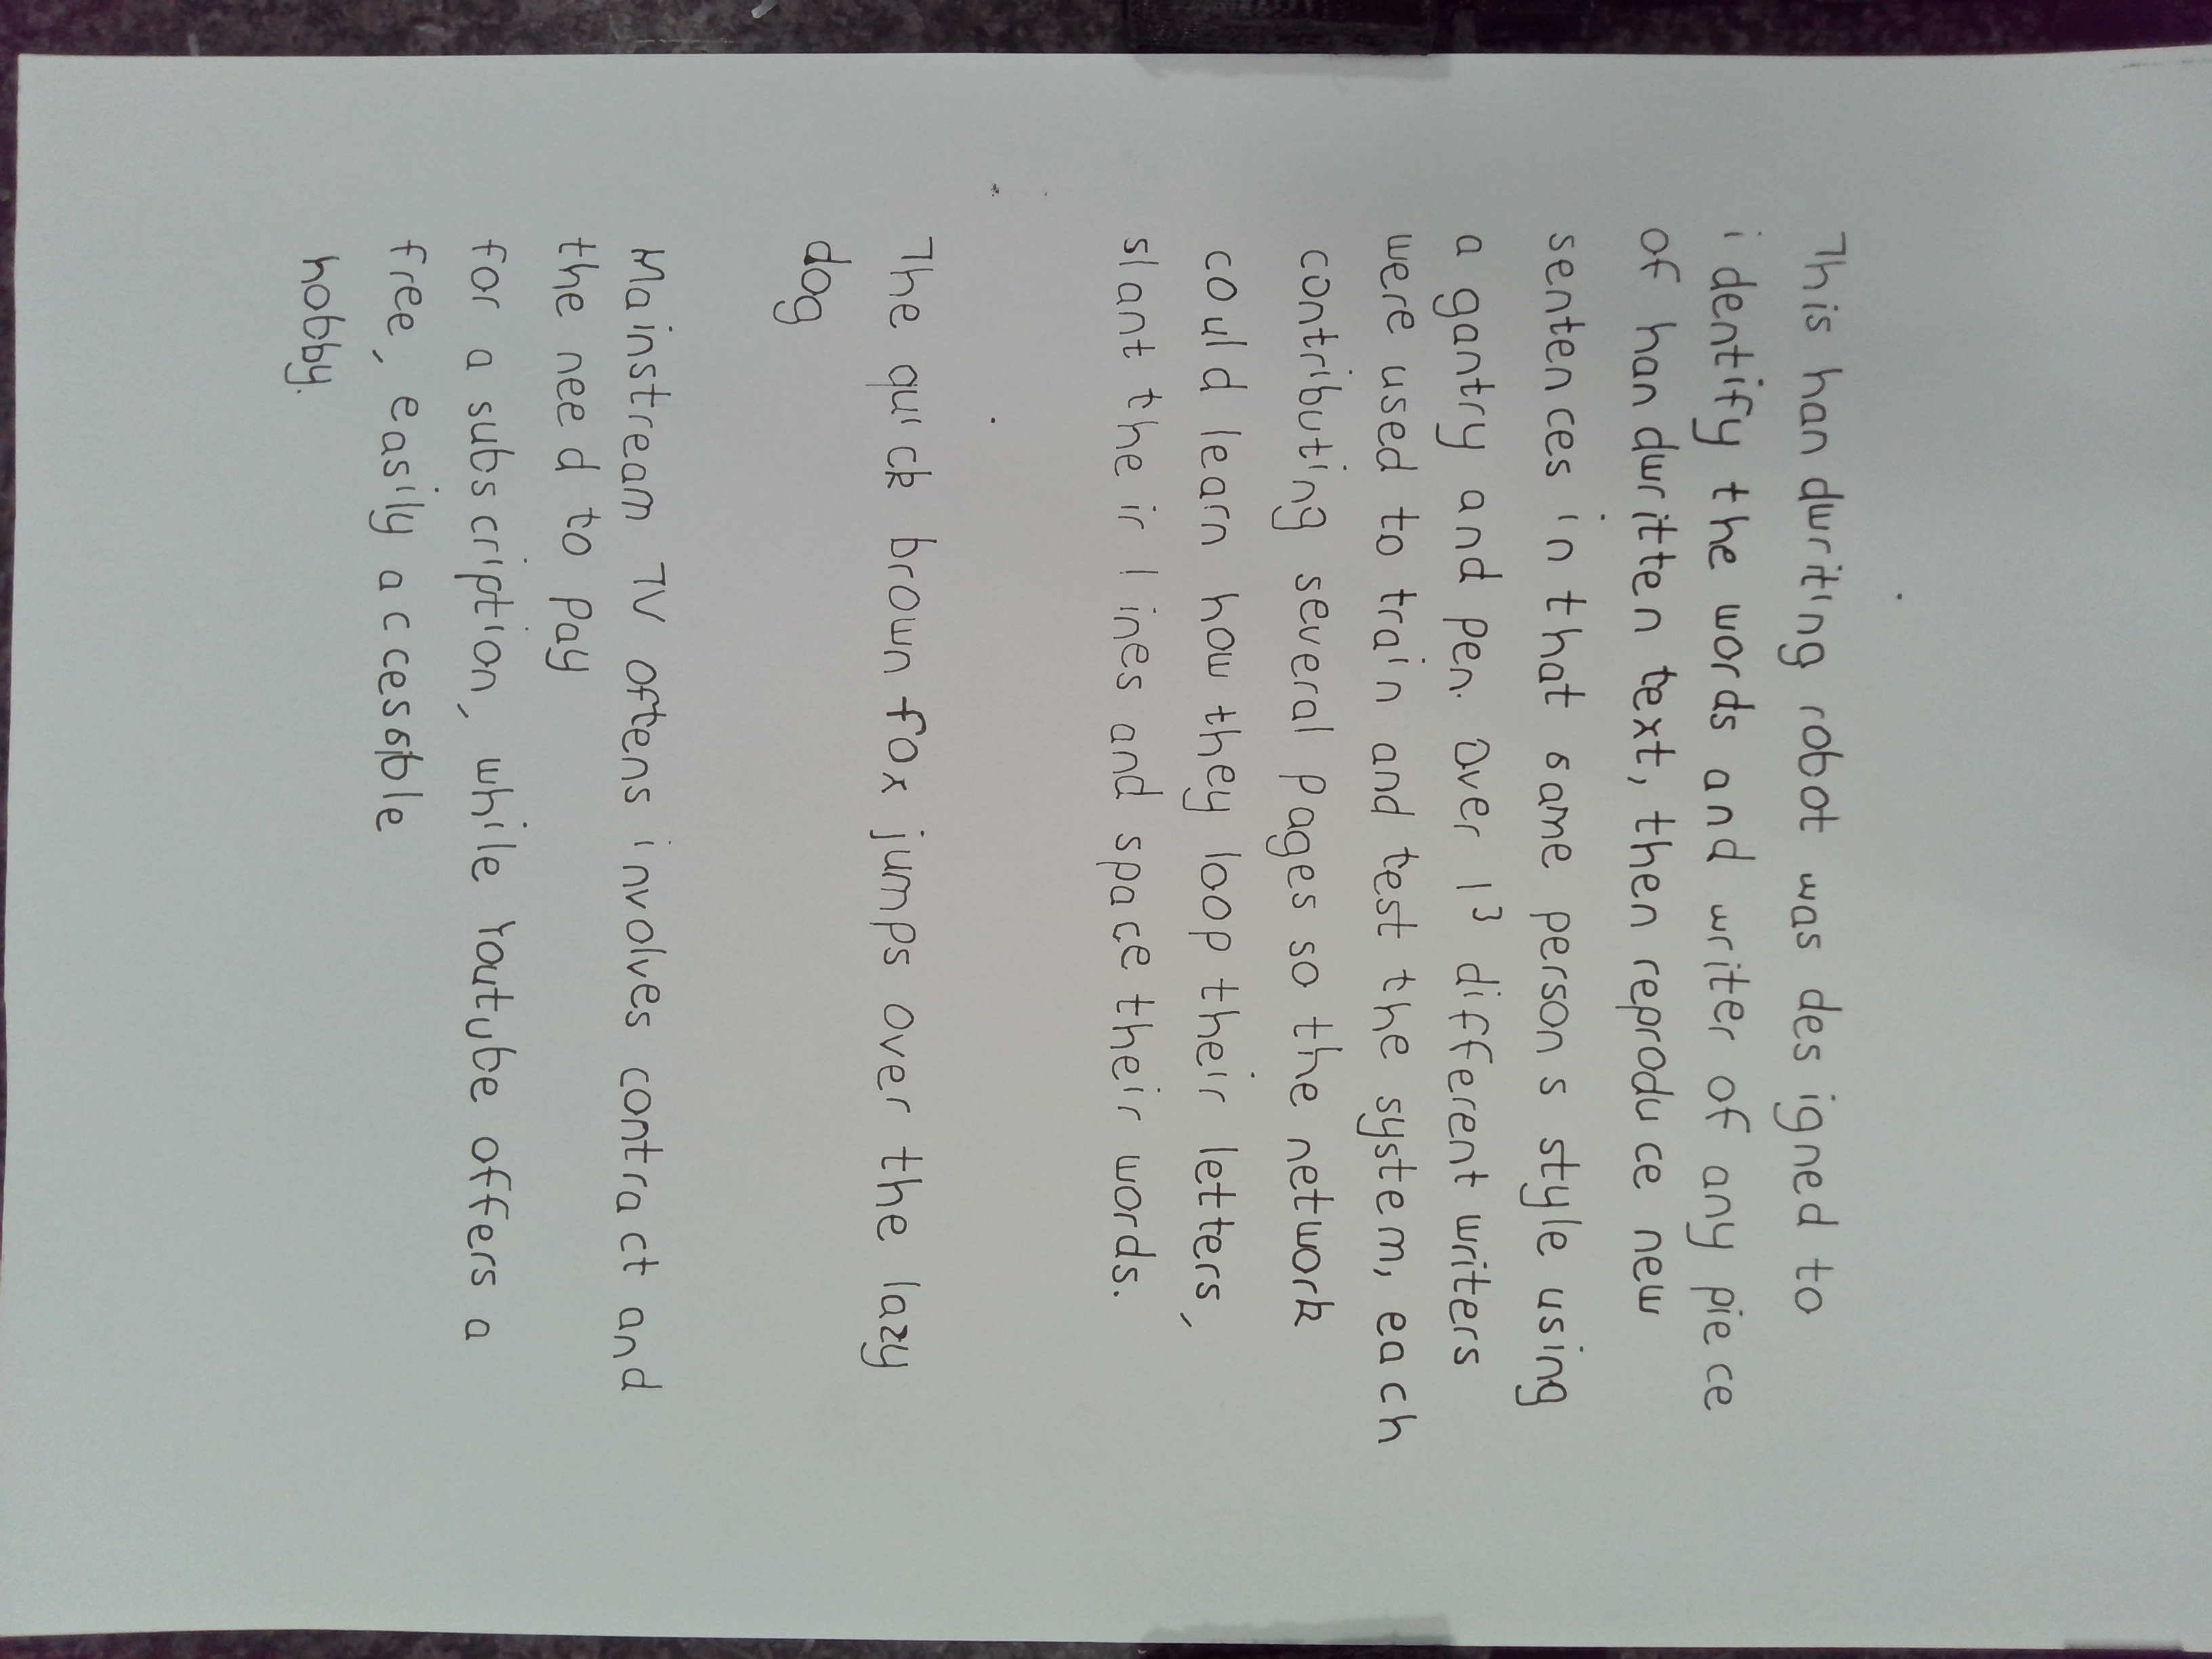
\includegraphics[angle=90,width=\linewidth,height=.55\textheight,keepaspectratio]{Figures/PhysicalPages/AuthorO.jpg}\par AuthorO\end{minipage}\hfill
\caption{Physical pages AuthorD, AuthorO.}\label{fig:app-physical-pages-6}\end{figure}
\begin{figure}[!htbp]\centering
\begin{minipage}{.48\linewidth}\centering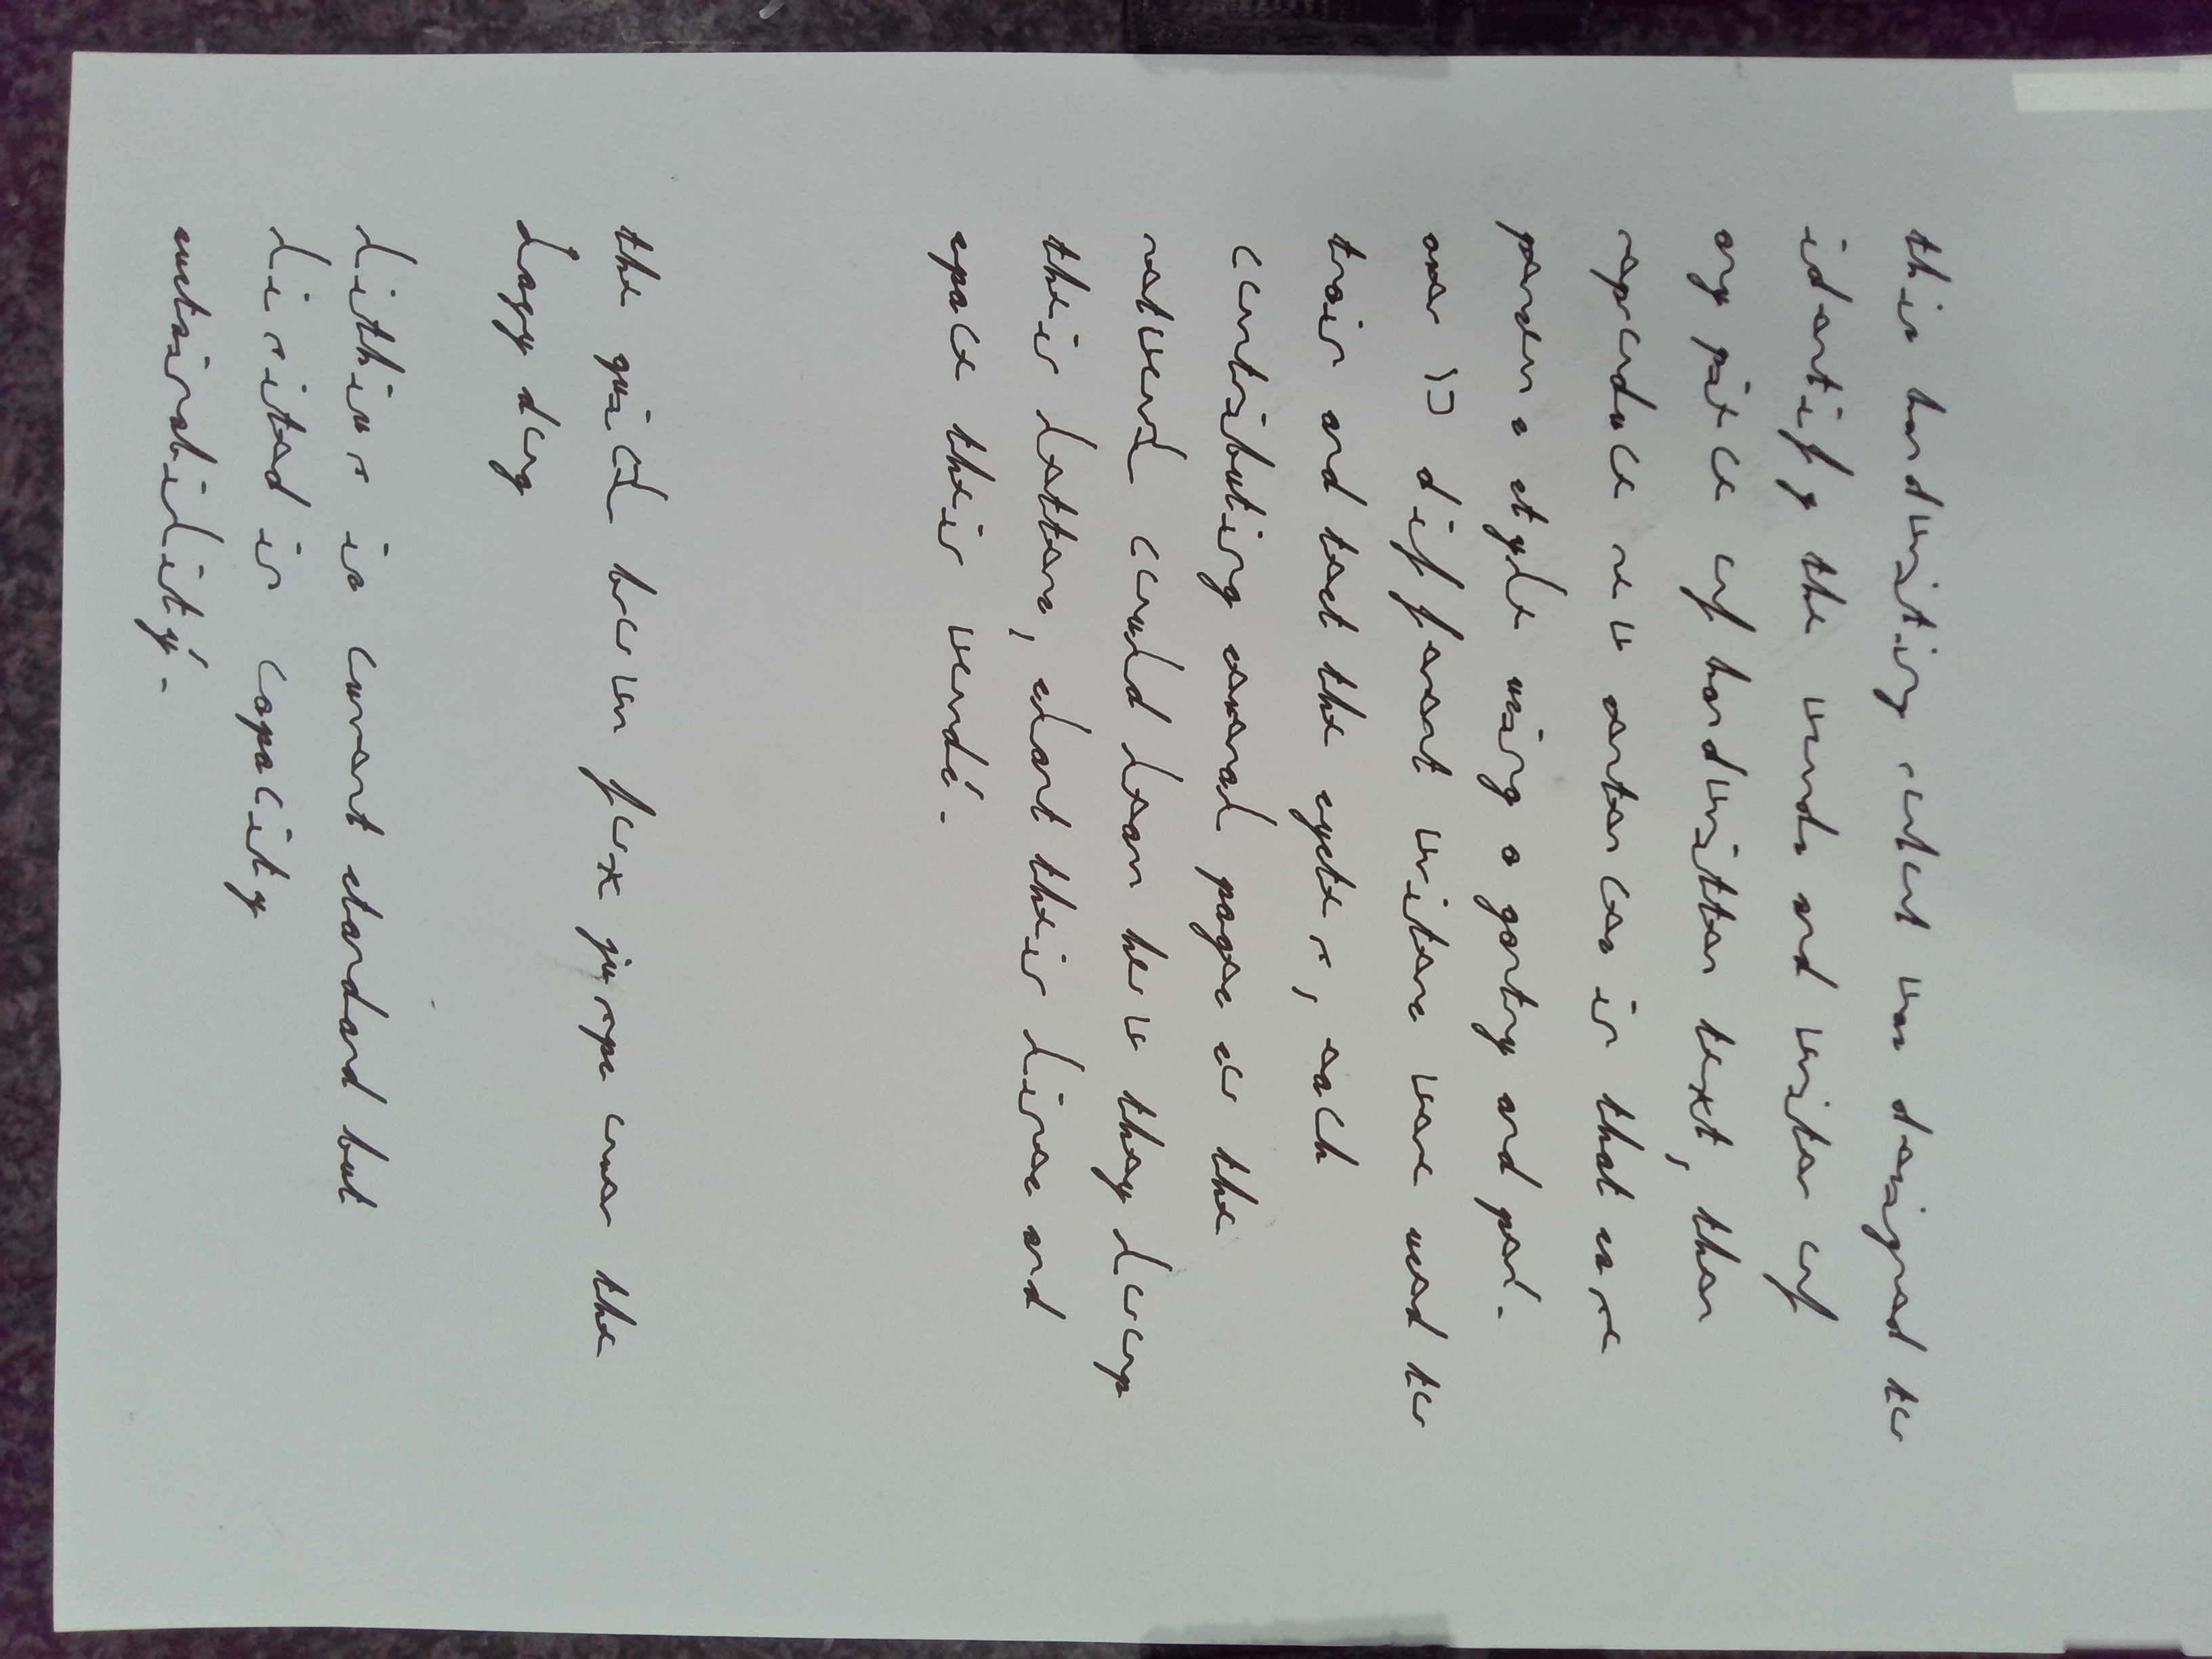
\includegraphics[angle=90,width=\linewidth,height=.55\textheight,keepaspectratio]{Figures/PhysicalPages/AuthorT.jpg}\par AuthorT\end{minipage}\hfill
\begin{minipage}{.48\linewidth}\centering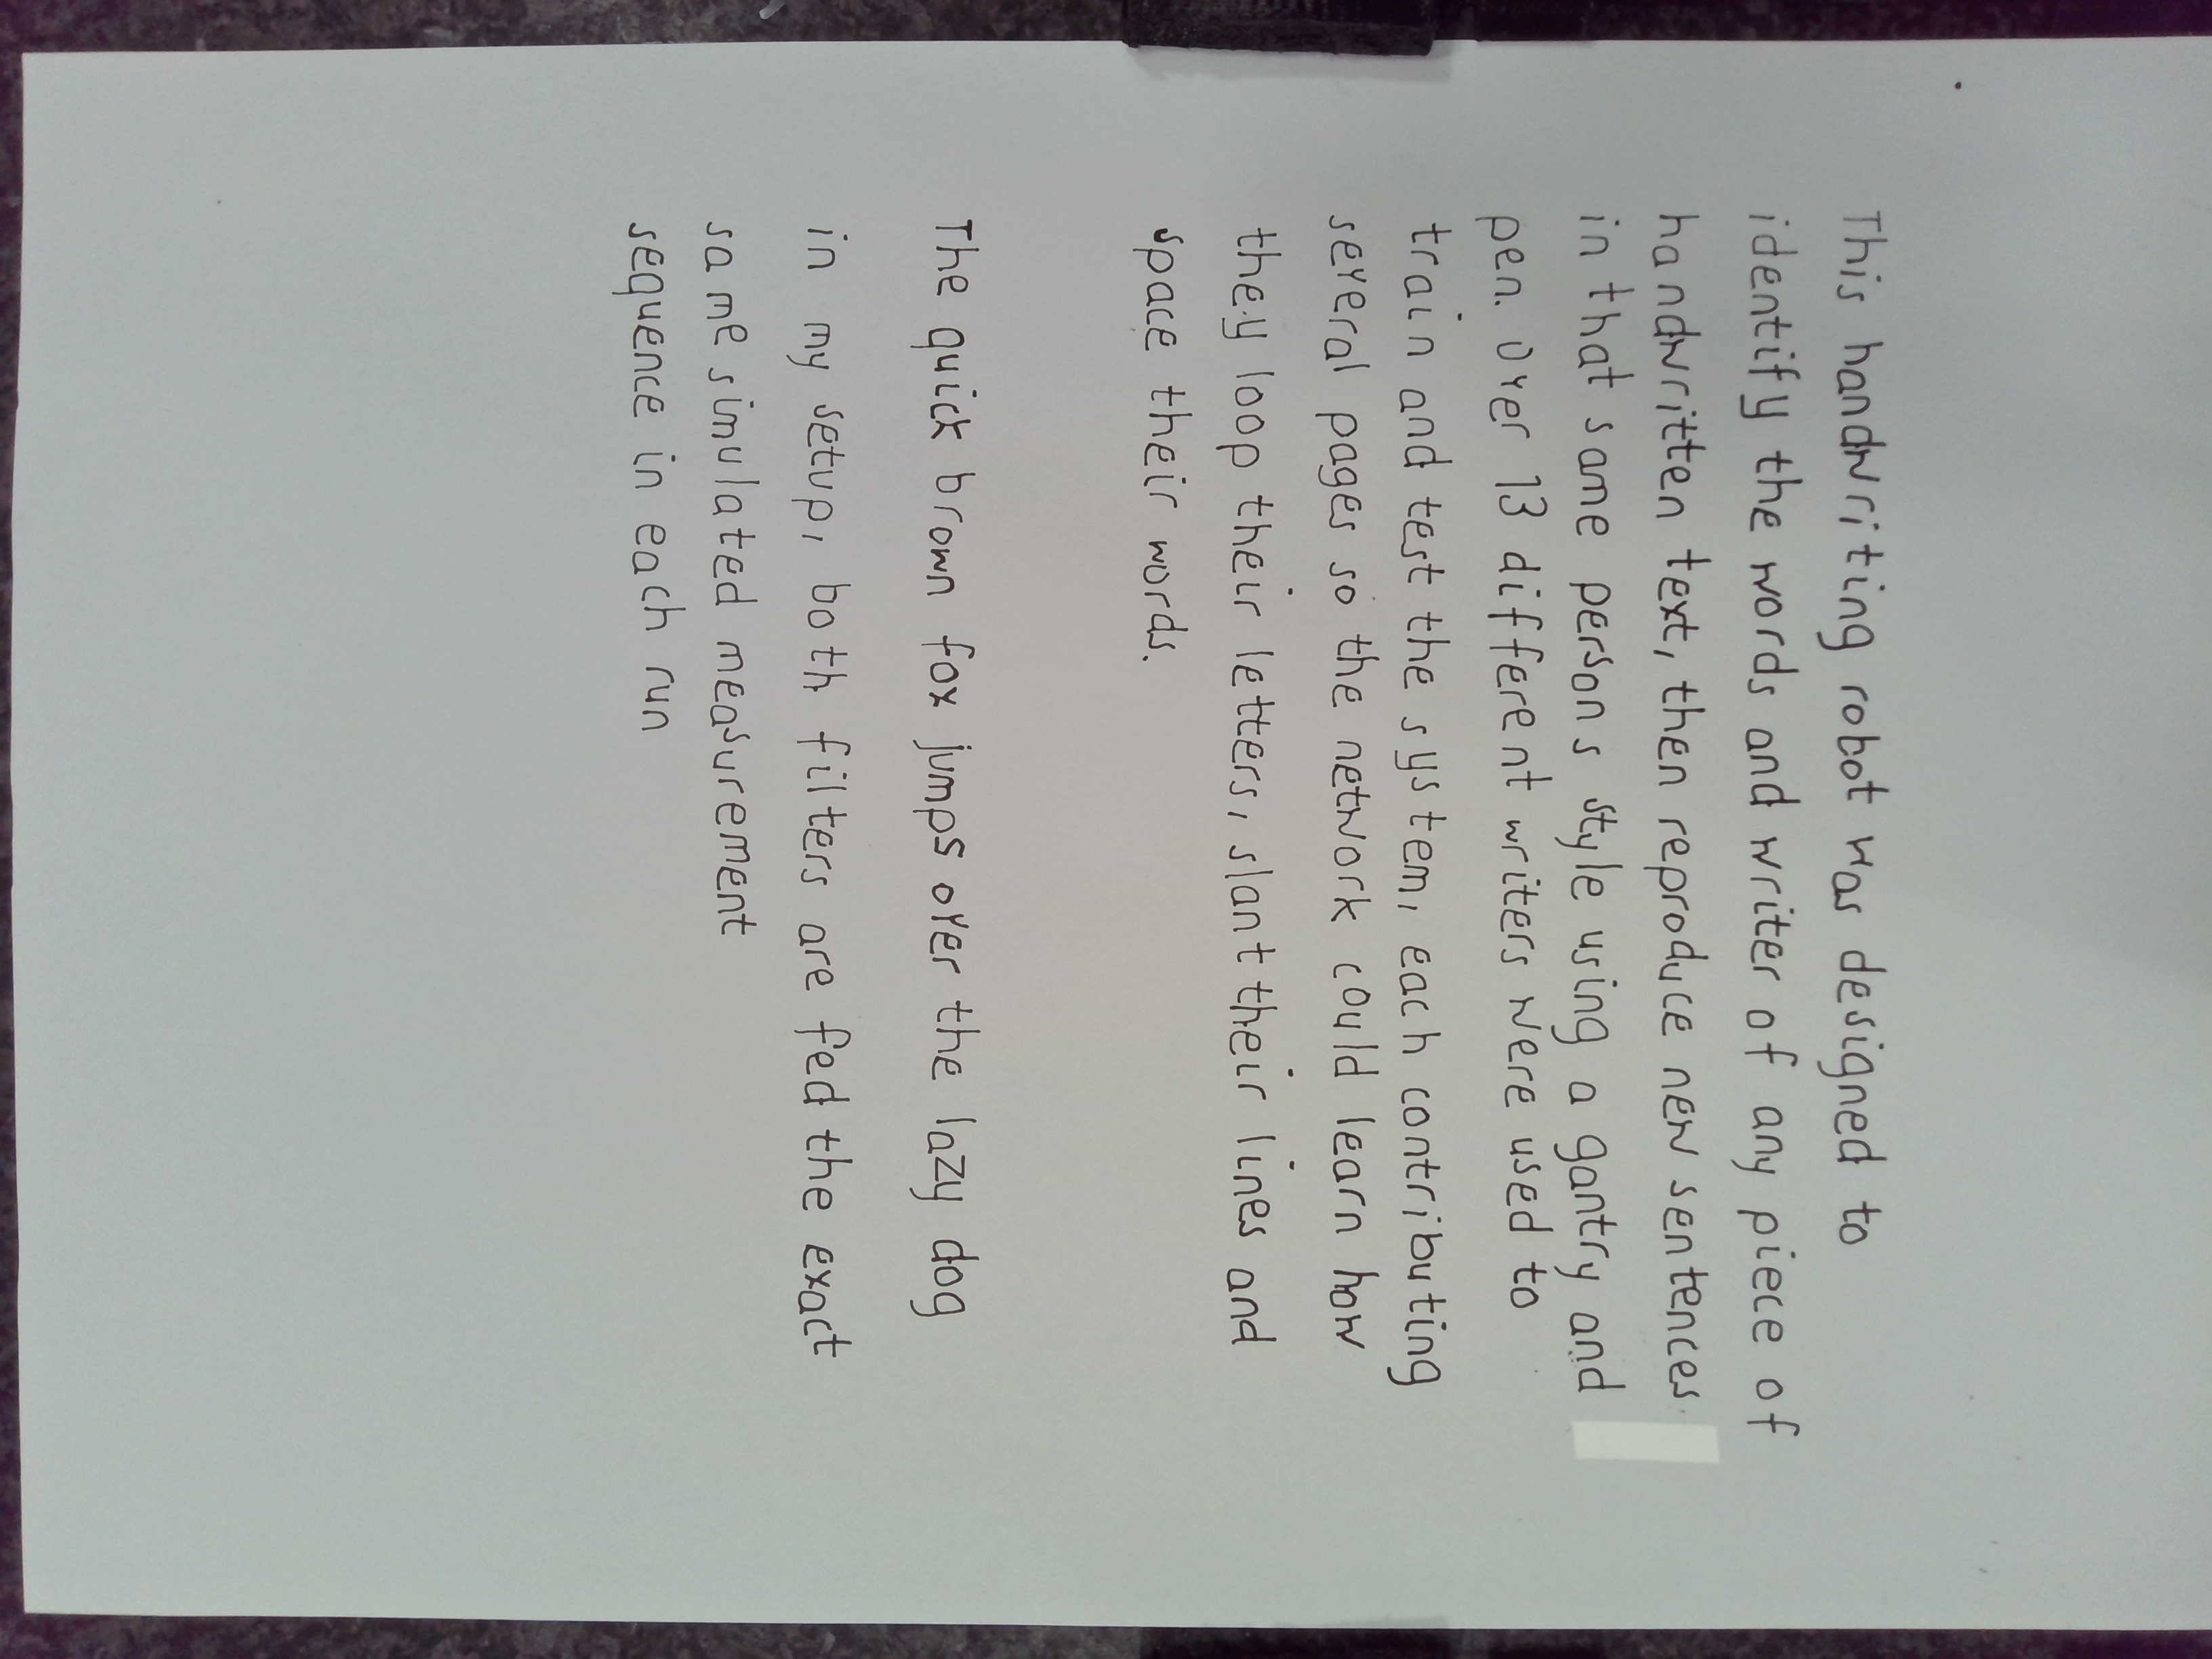
\includegraphics[angle=90,width=\linewidth,height=.55\textheight,keepaspectratio]{Figures/PhysicalPages/AuthorY.jpg}\par AuthorY\end{minipage}\hfill
\caption{Physical pages AuthorT, AuthorY.}\label{fig:app-physical-pages-7}\end{figure}
\FloatBarrier
